\documentclass[a4paper,11pt,openany]{report}
\usepackage{CJKutf8}

\usepackage[a4paper,margin=2.25cm,headheight=15pt]{geometry}
\usepackage{amsmath,amssymb,booktabs,longtable,tabularx,array,multirow}
\usepackage{graphicx,float,caption,subcaption,placeins}
\usepackage{xcolor,hyperref,fancyhdr,enumitem,titlesec}

\definecolor{atlasblue}{HTML}{163A5F}
\definecolor{atlaslight}{HTML}{EAF1F7}
\definecolor{goodgreen}{HTML}{1B7F5A}
\definecolor{warnorange}{HTML}{B35A00}
\hypersetup{colorlinks=true,linkcolor=atlasblue,urlcolor=atlasblue,citecolor=atlasblue}
\captionsetup{font=small,labelfont=bf}
\setlength{\parindent}{2em}
\setlength{\parskip}{0.35em}
\setlist[itemize]{leftmargin=2em,itemsep=0.25em}
\pagestyle{fancy}
\fancyhf{}
\fancyhead[L]{逐笔成交量化研究报告}
\fancyhead[R]{七因子与 Walk-forward LSTM}
\fancyfoot[C]{\thepage}
\titleformat{\chapter}[hang]{\huge\bfseries\color{atlasblue}}{\thechapter}{1em}{}
\titlespacing*{\chapter}{0pt}{-0.5em}{1.1em}

\newcommand{\pct}[1]{#1\%}
\newcommand{\code}[1]{\texttt{#1}}
\newcommand{\stepbox}[1]{%
  \begin{center}
  \colorbox{atlaslight}{\parbox{0.93\textwidth}{\textbf{#1}}}
  \end{center}}

\title{\textbf{逐笔成交数据、七因子选股与分钟级预测}\\[0.4em]
\large 数据处理、因子评价、换手控制回测与 Walk-forward LSTM}
\author{课程项目报告}
\date{2026 年 8 月 3 日}

\begin{document}
\begin{CJK*}{UTF8}{gbsn}
\renewcommand{\contentsname}{目录}
\renewcommand{\abstractname}{摘要}
\renewcommand{\figurename}{图}
\renewcommand{\tablename}{表}

\maketitle

\begin{abstract}
本项目完成了从逐笔成交数据到日频与分钟频数据、七因子构建与评价、执行约束组合回测，以及分钟级 LSTM 预测的完整研究流程。样本包含 300 只匿名股票和 302 个交易日。正式组合只使用截至上一交易日的历史信息，以 Top30、每 5 日调仓和 Top60 持有缓冲降低换手；次日开盘口径在卖出手续费、双边滑点、平方根冲击、停牌和涨跌停限制全部生效后，完整样本累计收益为 \textbf{32.74\%}，年化收益为 \textbf{29.51\%}，最大回撤为 \textbf{-11.27\%}，夏普率为 \textbf{1.494}。最后 20\% 留出期绝对收益为 -2.61\%，但同期等权基准为 -7.61\%，累计主动收益为 5.41\%。因此，完整样本结果说明策略具有研究价值，但不能被解释为未来收益保证。
\end{abstract}

\tableofcontents
\clearpage

\chapter{研究目标与总体流程}

本项目围绕三个问题展开：第一，逐笔成交数据能否被无前视地加工成可复用的日频和分钟频数据；第二，七个横截面因子是否具有预测下一交易日收益的能力，并能否在真实交易约束下产生超额收益；第三，LSTM 是否能在严格的时间序列样本外验证中提供简单逻辑回归之外的分钟级排序信息。

\stepbox{流程 1：逐笔成交清洗 $\rightarrow$ 日频/分钟频聚合 $\rightarrow$ 七因子构建 $\rightarrow$ 因子评价 $\rightarrow$ 历史 IC 加权 $\rightarrow$ 执行约束回测 $\rightarrow$ 稳健性分析 $\rightarrow$ Walk-forward LSTM。}

为避免结果“看起来很好但无法交易”，报告把预测能力、执行成本和样本外表现分开评价。所有正式策略统计均来自非前视版本 \code{historical\_20d\_ic}；使用同日未来收益的版本只用于展示数据泄漏，不计入正式结论。

\chapter{数据处理：从逐笔成交到标准面板}

\section{步骤一：读取、排序与基础校验}

逐笔文件首先按股票、交易日和成交时间排序，并检查价格、成交量、买卖方向和复权因子的类型与缺失情况。项目覆盖 300 只股票、302 个交易日。分钟时间轴固定包含集合竞价、上午与下午连续竞价以及 15:00 收盘分钟，每日共 253 个时间点。

输出的 11 个基础字段为：开盘价、最高价、最低价、收盘价、成交量、成交笔数、成交额、主动买量、主动卖量、主动买额和主动卖额。价格字段形成日频宽表与逐日分钟宽表；最终另生成 90,600 行的日频 K 线长表，供因子与回测程序统一读取。

\section{步骤二：价格单位恢复与复权}

原始成交价格以乘 100 的整数保存，因此先恢复真实成交价格：
\begin{equation}
P^{\mathrm{real}}_{i,t}=\frac{P^{\mathrm{raw}}_{i,t}}{100}.
\end{equation}
随后对价格字段乘以当日复权因子 $F_{i,t}$：
\begin{equation}
P^{\mathrm{adj}}_{i,t}=P^{\mathrm{real}}_{i,t}\times F_{i,t}.
\end{equation}
复权价格用于跨日收益和技术类因子，以消除分红、送股等公司行为造成的机械跳变。成交额仍按真实未复权价格计算：
\begin{equation}
A_{i,t}=P^{\mathrm{real}}_{i,t}\times V_{i,t},
\end{equation}
因为成交额描述的是当时真实发生的交易金额，不应被复权因子改变。

\section{步骤三：OHLC 与买卖方向聚合}

每个日频或分钟频分组内，第一笔成交价为开盘价，最大值为最高价，最小值为最低价，最后一笔成交价为收盘价；成交量、成交笔数和成交额采用求和。买卖方向按 \code{BSFlag} 拆分：0 为主动买、1 为主动卖、2 为集合竞价，由此分别汇总主动买卖的量和金额。

\section{步骤四：无成交时点的填充}

价格只使用已经发生过的历史收盘价向后填充。日频缺失 OHLC 使用前一交易日收盘价，分钟频缺失 OHLC 使用前一分钟收盘价；在第一笔成交出现之前不使用当天未来成交价。没有成交的量、额和笔数统一填 0。这一规则避免了把未来价格填回过去分钟的前视偏差。

\chapter{七因子构建、公式与经济含义}

令 $A$ 为成交额，$V$ 为成交量，$N$ 为成交笔数，$O,H,L,C$ 分别为复权后的开盘、最高、最低和收盘价；$BVol$ 与 $SVol$ 为主动买量与主动卖量，$r^{cc}_t=C_t/C_{t-1}-1$。本项目使用以下七个因子。

\begin{longtable}{p{0.24\textwidth}p{0.39\textwidth}p{0.29\textwidth}}
\toprule
因子 & 公式 & 经济含义 \\
\midrule
\endfirsthead
\toprule
因子 & 公式 & 经济含义 \\
\midrule
\endhead
成交额多窗口均值离散度 & $\log\!\left(1+\mathrm{sd}(\overline A^{(1)},\overline A^{(5)},\overline A^{(10)},\overline A^{(20)})\right)$ & 衡量不同期限成交额均值的分化程度；数值大表示流动性状态变化更剧烈。\\
5 日主动买卖不平衡 & $\mathrm{MA}_5\!\left((BVol-SVol)/\max(V,1)\right)$ & 衡量主动买盘相对主动卖盘的持续强弱。\\
10 日日内振幅 & $\mathrm{MA}_{10}\!\left((H-L)/C\right)$ & 表示近期盘中波动和不确定性水平。\\
5 日反转 & $-\left(C_t/C_{t-5}-1\right)$ & 捕捉短期价格过度反应后的反转。\\
20 日单笔成交规模异常 & $z_{20}\!\left(\log(1+A/\max(N,1))\right)$ & 识别平均单笔成交金额相对自身历史的异常变化。\\
10 日价量压力 & $\mathrm{MA}_{10}\!\left(r^{cc}_t\,\Delta\log(1+V_t)\right)$ & 联合刻画价格方向与成交量变化，区分放量上涨和放量下跌。\\
5 日隔夜--日内收益背离 & $\mathrm{MA}_5\!\left[(O_t/C_{t-1}-1)-(C_t/O_t-1)\right]$ & 比较隔夜跳空与日内价格兑现方向，刻画两类交易时段的信息分歧。\\
\bottomrule
\end{longtable}

\section{步骤五：横截面预处理}

每天对每个因子进行 1\% 和 99\% 分位缩尾，再做横截面标准化：
\begin{equation}
z_{i,t}=\frac{x_{i,t}-\bar x_t}{s_t}.
\end{equation}
程序预留了行业与市值中性化接口，即把因子对行业哑变量及标准化后的对数市值做横截面回归并使用残差。但匿名数据没有提供真实行业和市值，因此本次运行状态记录为 \code{SKIPPED\_NO\_EXPOSURES}，不使用虚构代理变量。

\chapter{因子评价与图像解释}

\section{步骤六：IC、Rank IC 与分组收益}

评价目标为下一交易日收盘到收盘收益。普通 IC 是当日因子与下一日收益的 Pearson 相关系数；Rank IC 是二者秩的 Spearman 相关系数。报告同时计算均值、波动和 ICIR：
\begin{equation}
\mathrm{ICIR}=\frac{\overline{\mathrm{IC}}}{\sigma(\mathrm{IC})}.
\end{equation}
五分组检验将每日股票按因子从低到高分为 Q1--Q5，比较组间平均收益、累计净值与 Q5--Q1 多空收益。若因子呈负向预测，则综合策略会根据历史 IC 自动反转其方向。

\begin{table}[H]
\centering
\small
\caption{七因子评价汇总}
\begin{tabular}{lrrrr}
\toprule
因子 & IC & Rank IC & Rank ICIR & Q5--Q1 累计收益 \\
\midrule
成交额多窗口均值离散度 & -0.0774 & -0.1070 & -11.711 & -75.86\% \\
5 日主动买卖不平衡 & 0.0016 & -0.0017 & -0.266 & 3.03\% \\
10 日日内振幅 & -0.0396 & -0.0783 & -6.871 & -41.95\% \\
5 日反转 & 0.0303 & 0.0558 & 6.357 & 50.53\% \\
20 日单笔成交规模异常 & -0.0225 & -0.0500 & -8.536 & -36.25\% \\
10 日价量压力 & -0.0424 & -0.0752 & -10.354 & -51.65\% \\
5 日隔夜--日内收益背离 & 0.0324 & 0.0539 & 7.187 & 80.41\% \\
\bottomrule
\end{tabular}
\end{table}

每张诊断图按同一方式阅读：左上为 Q1--Q5 平均收益，用于检查单调性；右上为各分组累计净值；左下为 Q5--Q1 多空净值；右下为滚动 Rank IC，用于观察稳定性和阶段性失效。

\begin{figure}[H]\centering
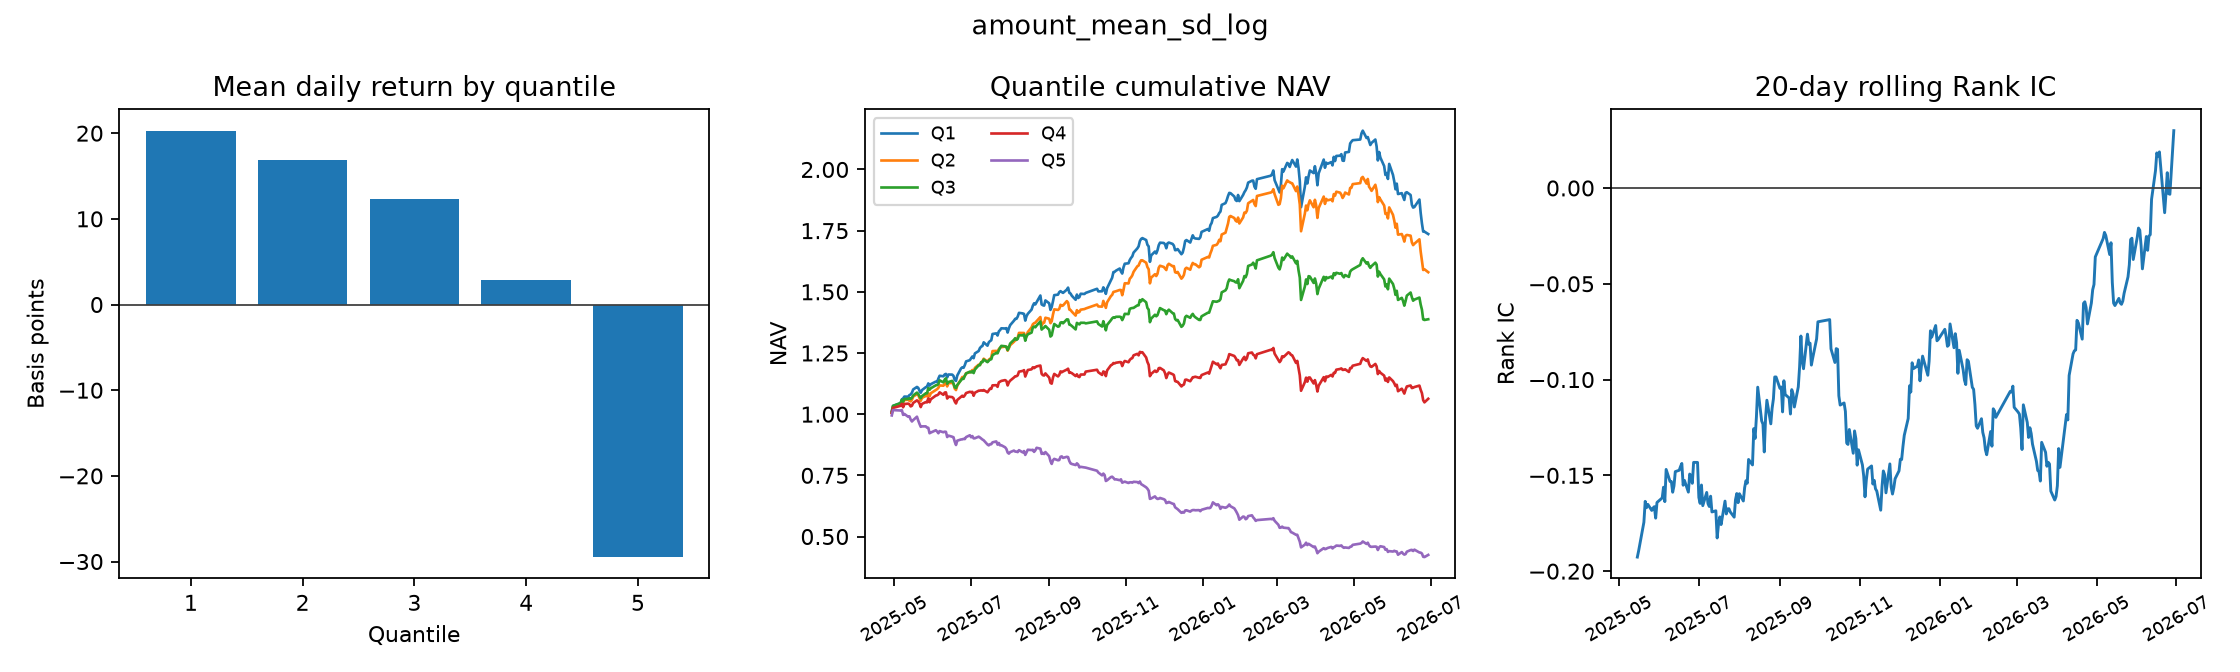
\includegraphics[width=0.96\textwidth]{qr_factor_amount.png}
\caption{成交额多窗口均值离散度因子诊断。负 Rank IC 和下降的分组收益说明该因子应反向使用。}
\end{figure}

\begin{figure}[H]\centering
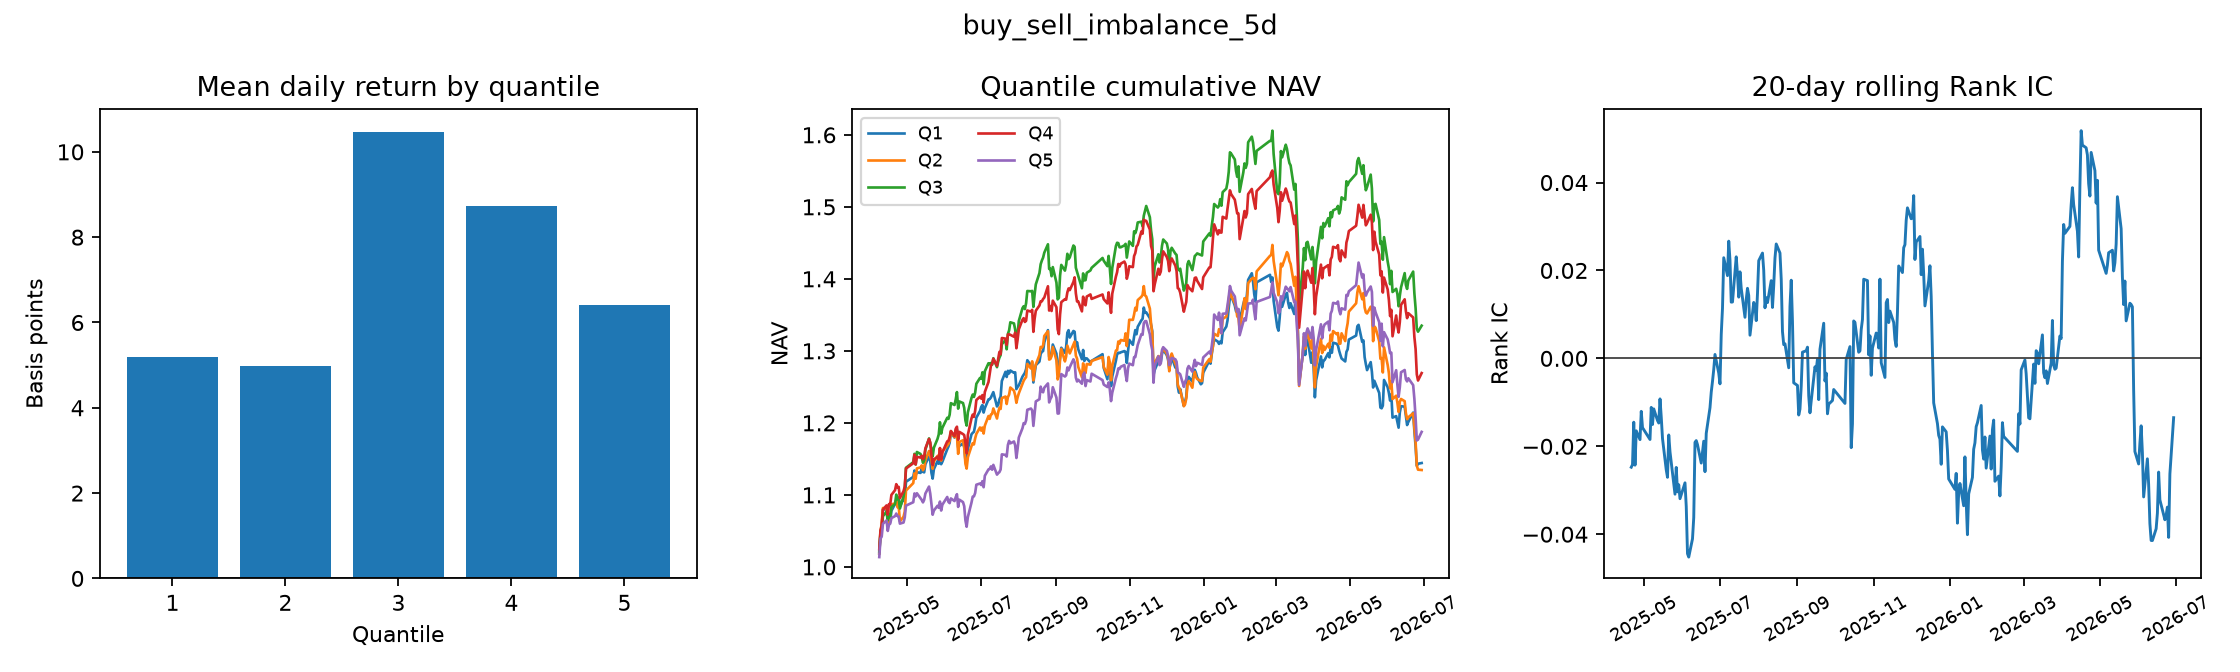
\includegraphics[width=0.96\textwidth]{qr_factor_imbalance.png}
\caption{主动买卖不平衡因子诊断。其 Rank IC 接近零，单因子预测力较弱，因此不应单独承担组合方向。}
\end{figure}

\begin{figure}[H]\centering
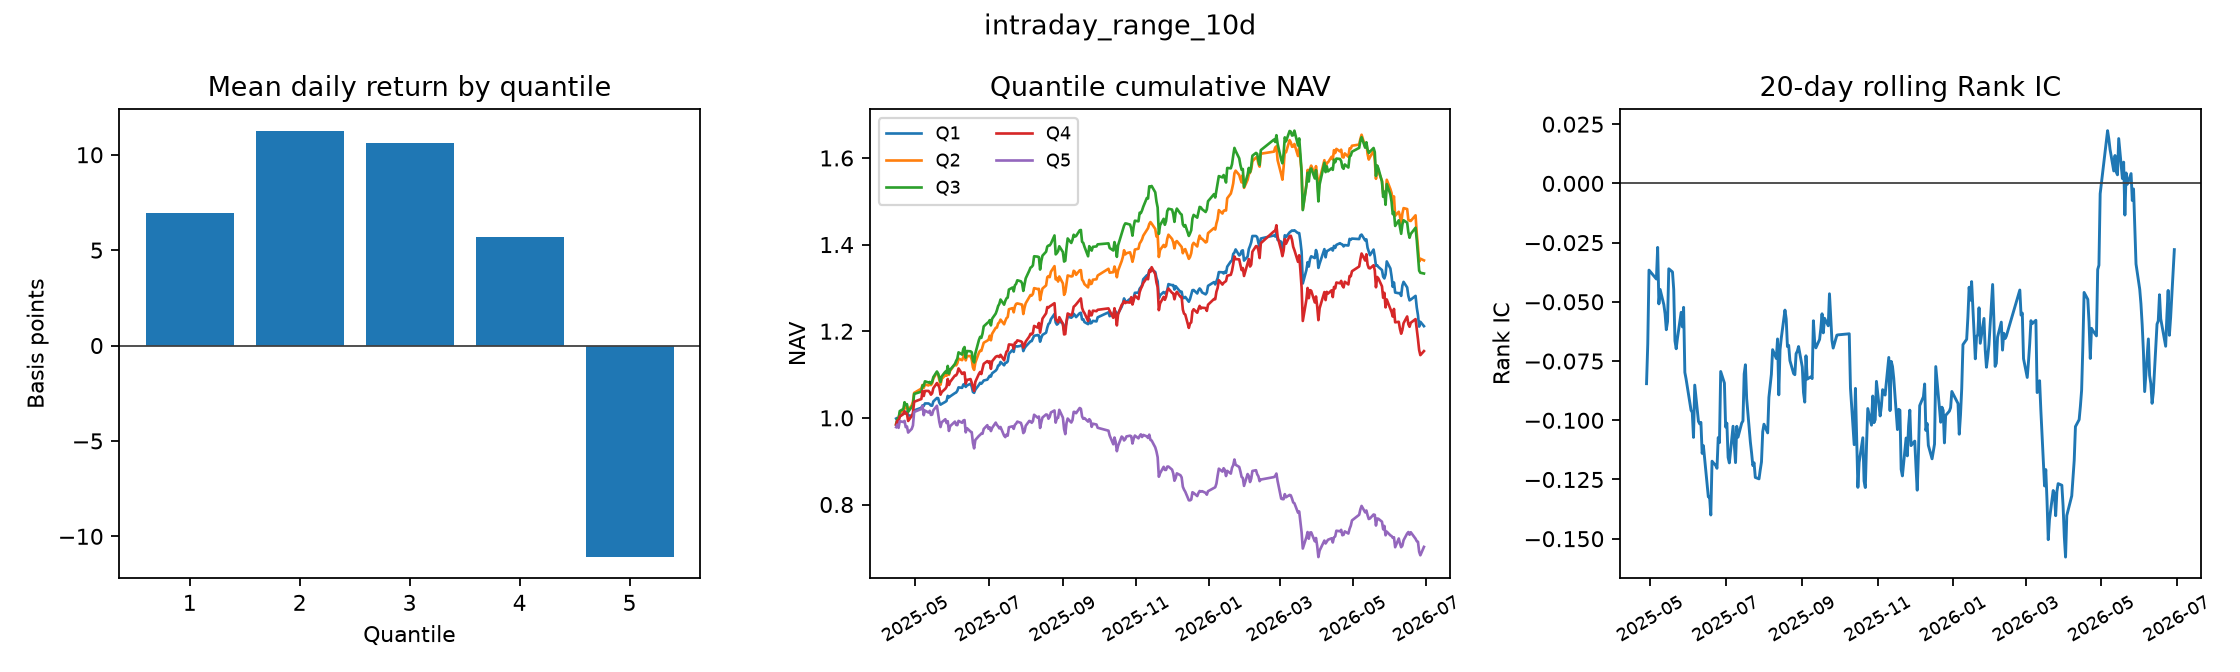
\includegraphics[width=0.96\textwidth]{qr_factor_range.png}
\caption{日内振幅因子诊断。高振幅组未来收益较弱，表现为稳定的负向因子。}
\end{figure}

\begin{figure}[H]\centering
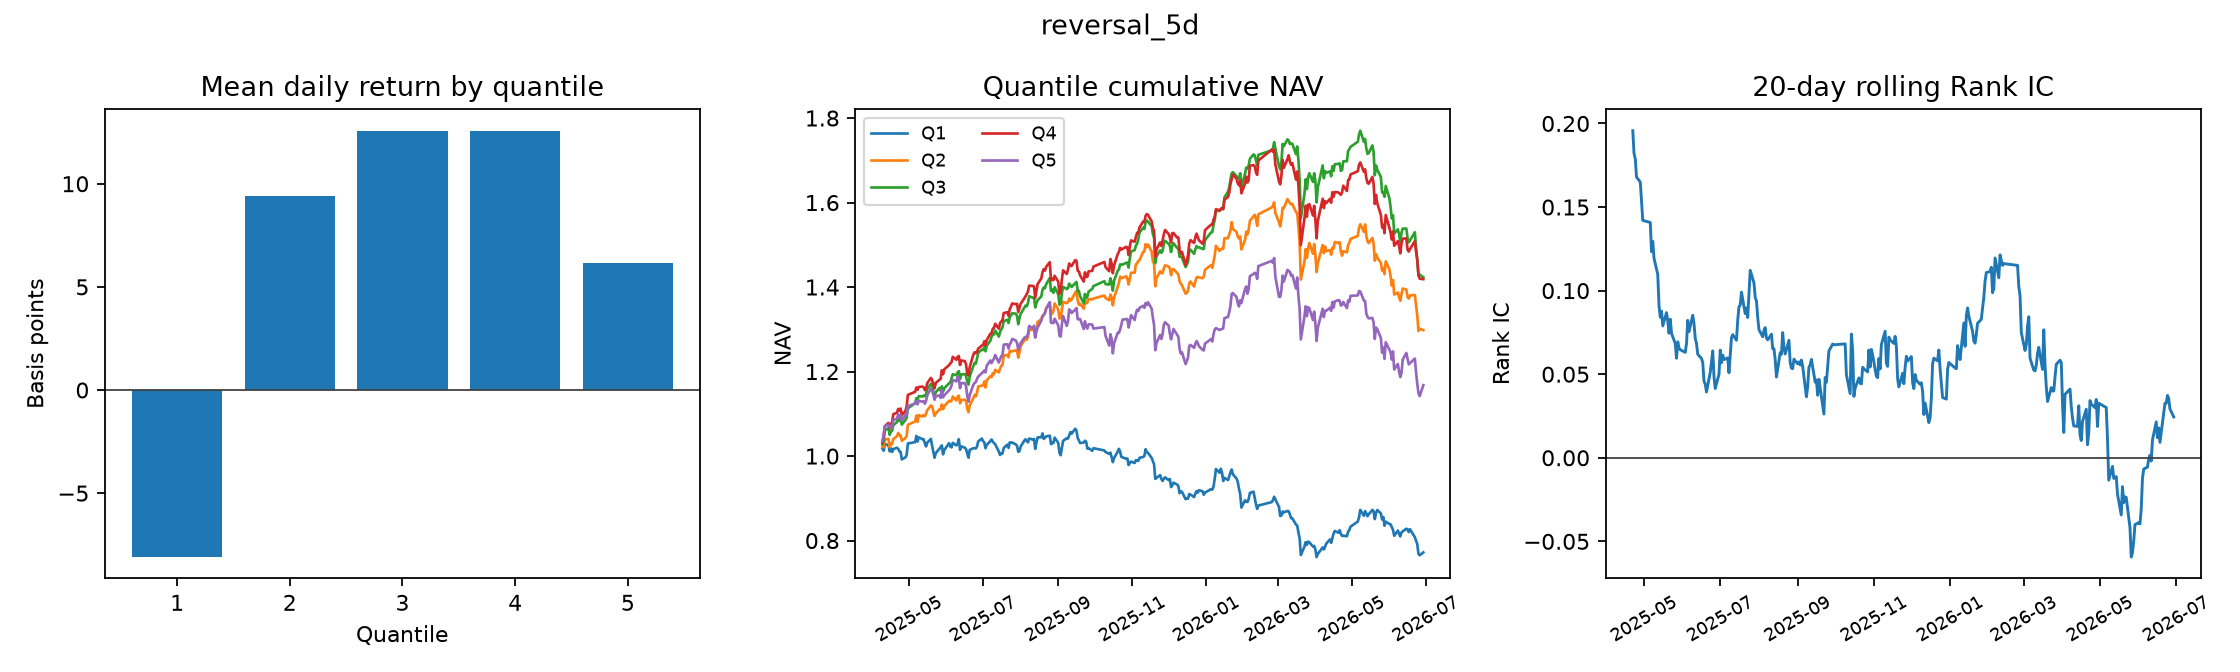
\includegraphics[width=0.96\textwidth]{qr_factor_reversal.png}
\caption{5 日反转因子诊断。正 Rank IC 与正多空收益表明近期弱势股票随后存在一定反弹。}
\end{figure}

\begin{figure}[H]\centering
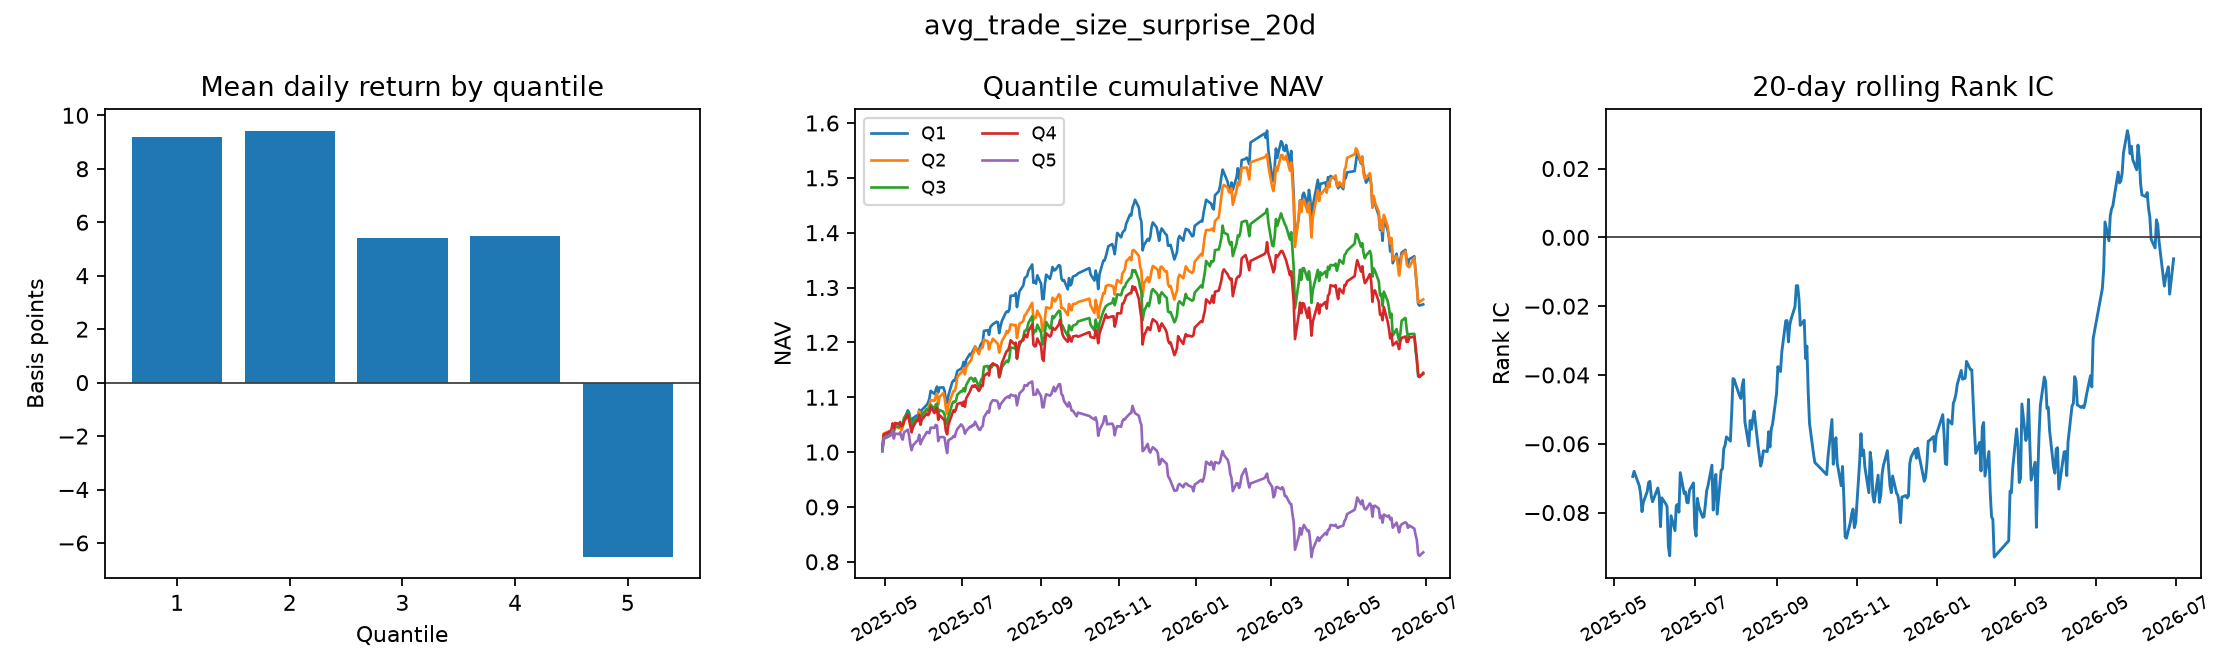
\includegraphics[width=0.96\textwidth]{qr_factor_trade_size.png}
\caption{20 日单笔成交规模异常因子诊断。异常放大的平均单笔成交规模与下一日收益呈负相关。}
\end{figure}

\begin{figure}[H]\centering
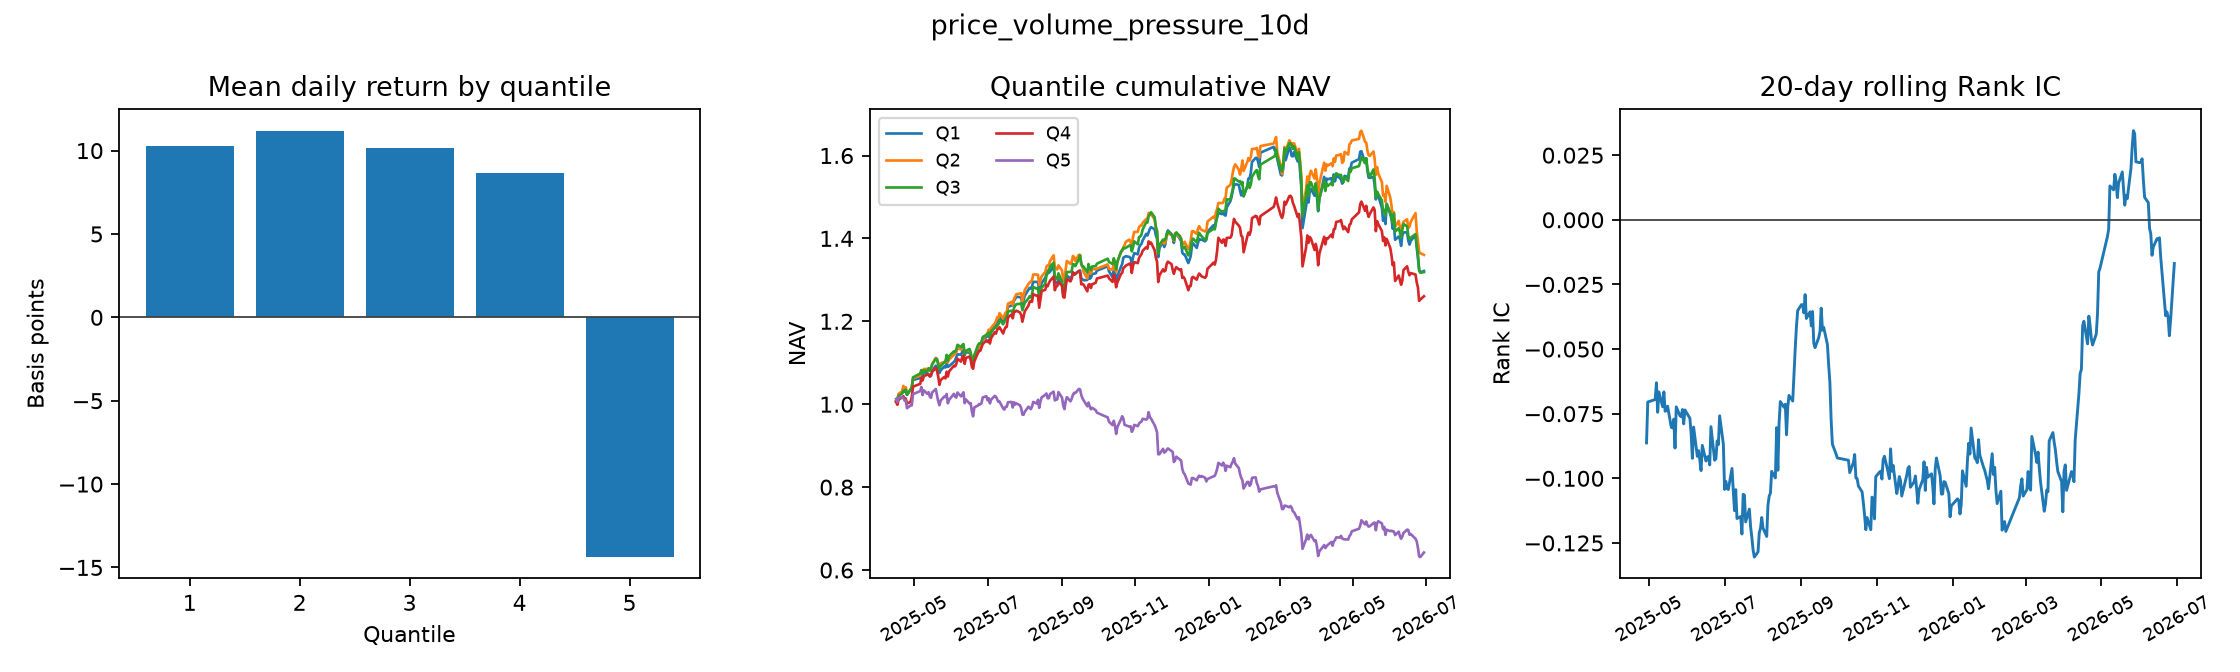
\includegraphics[width=0.96\textwidth]{qr_factor_price_volume.png}
\caption{10 日价量压力因子诊断。该因子呈负向预测，显示近期价量同向压力可能伴随后续修正。}
\end{figure}

\begin{figure}[H]\centering
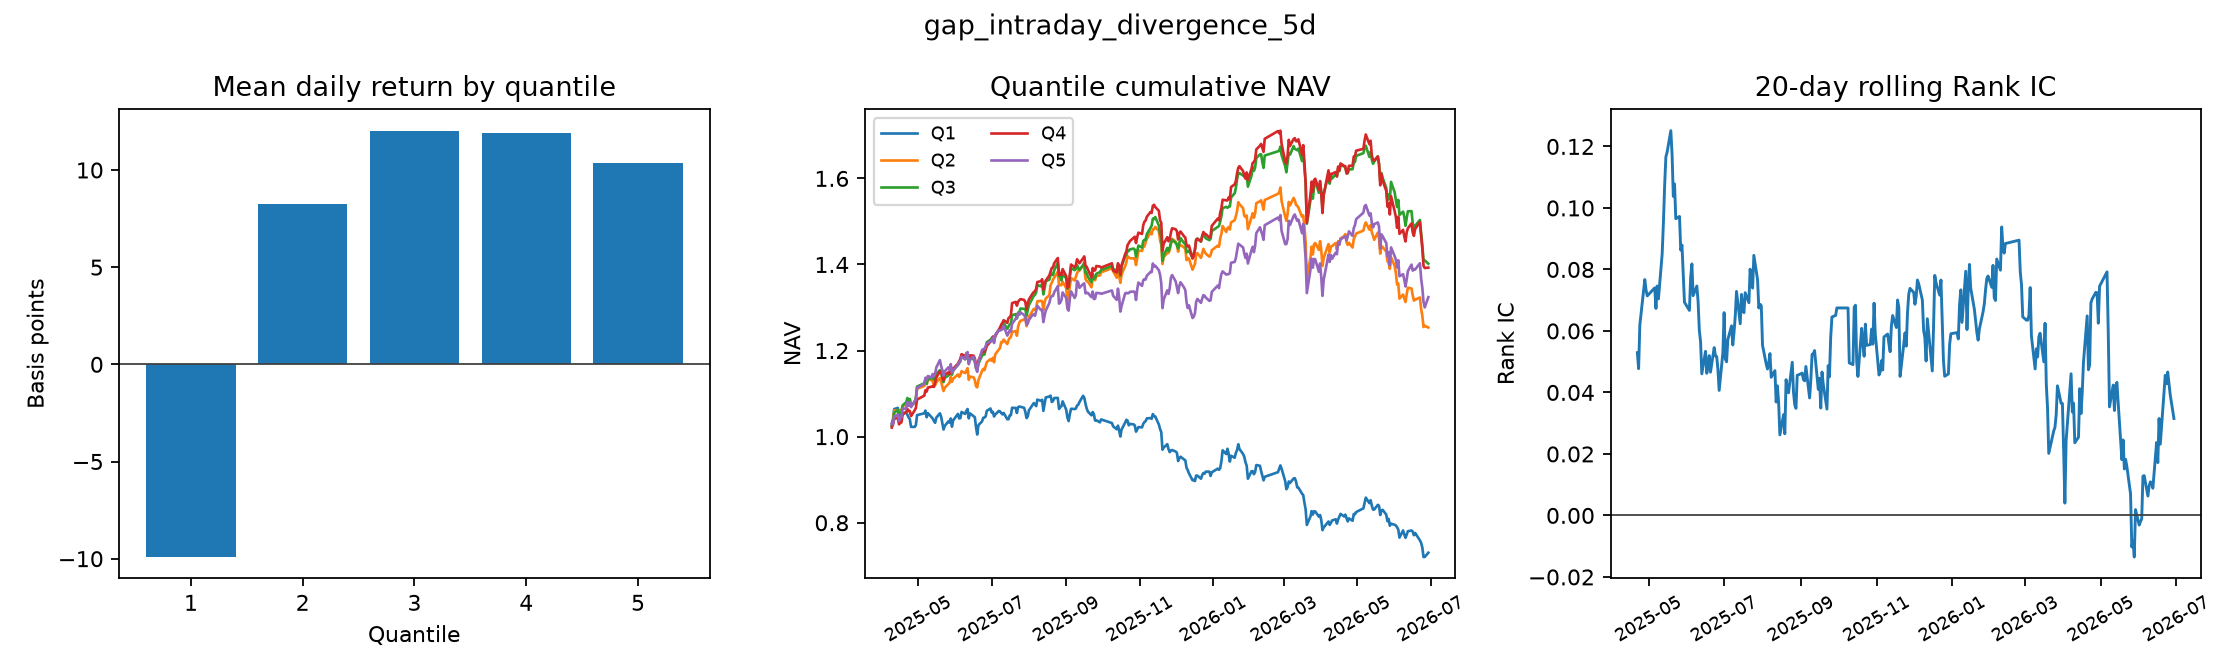
\includegraphics[width=0.96\textwidth]{qr_factor_gap_intraday.png}
\caption{5 日隔夜--日内收益背离因子诊断。其 Q5--Q1 累计收益为 80.41\%，是新增因子中表现最强的一项。}
\end{figure}

\section{步骤七：相关性与多空净值}

因子相关性用于识别重复信息。最大绝对相关性约为 0.535，出现在隔夜--日内背离与 5 日反转之间；其余组合并未达到完全共线。新增因子在组合中使用保守信号乘数，防止短样本中的强 IC 直接主导权重。

\begin{figure}[H]\centering
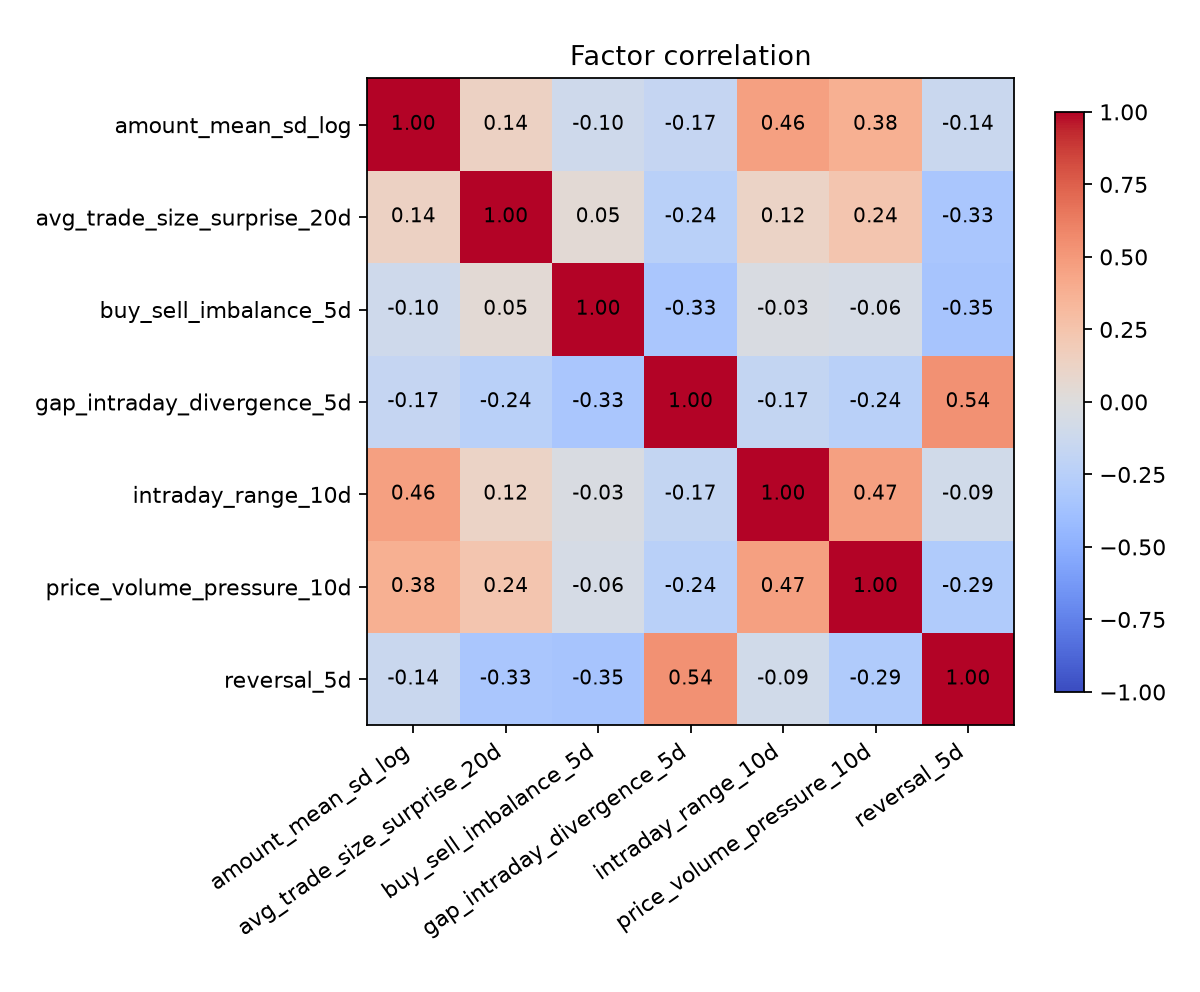
\includegraphics[width=0.86\textwidth]{qr_factor_corr.png}
\caption{七因子横截面相关系数热力图。}
\end{figure}

\begin{figure}[H]\centering
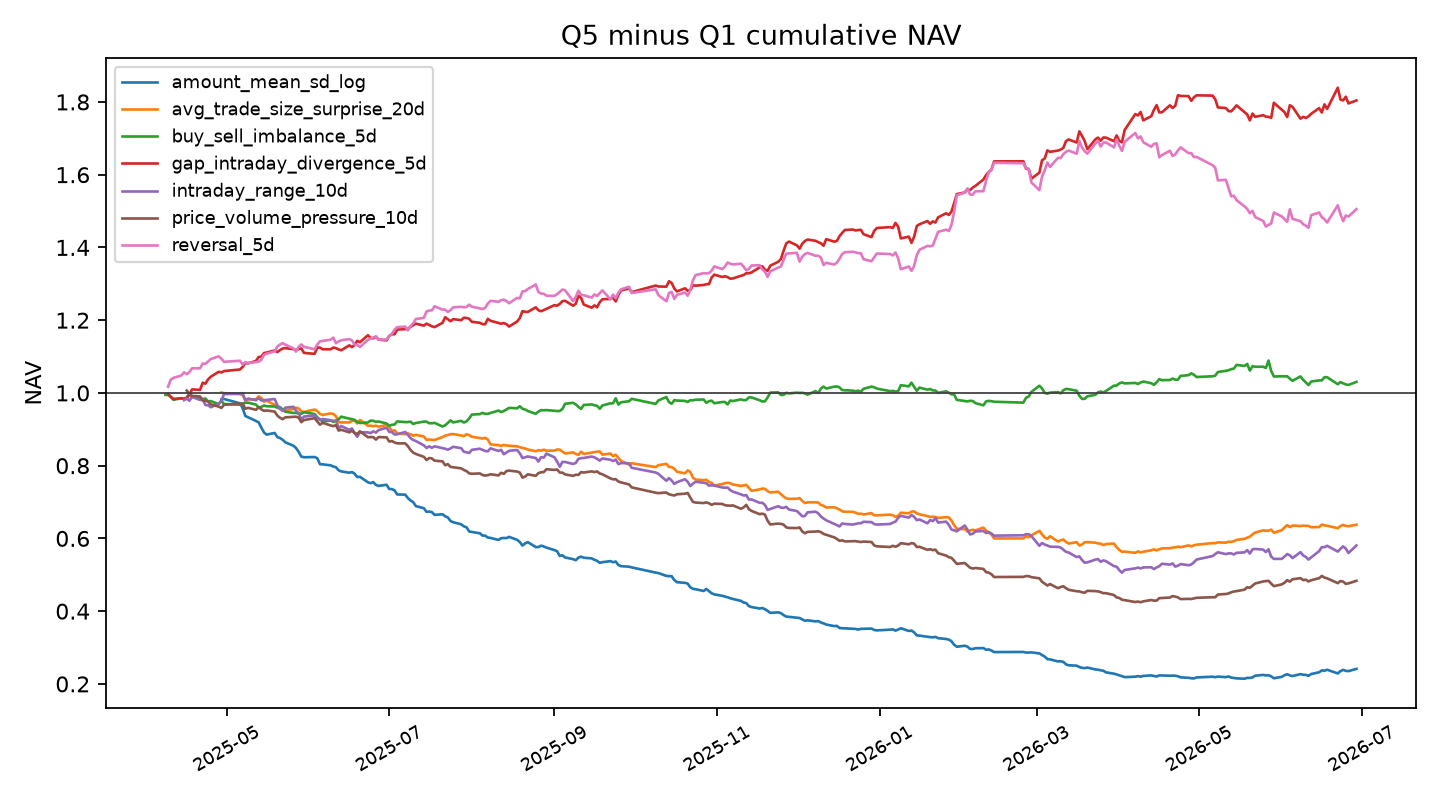
\includegraphics[width=0.94\textwidth]{qr_factor_ls_nav.png}
\caption{七因子 Q5--Q1 多空累计净值。正负方向不同的因子在组合前按历史 IC 调整方向。}
\end{figure}

\chapter{组合构建与无前视回测}

\section{步骤八：历史 IC 加权形成综合信号}

因子 $k$ 在交易日 $t$ 的方向和权重只使用截至 $t-1$ 的 20 日历史 IC：
\begin{equation}
\bar{IC}_{k,t}=\frac{1}{20}\sum_{s=t-20}^{t-1}IC_{k,s},\qquad
w_{k,t}=\frac{\bar{IC}_{k,t}}{\sum_j |\bar{IC}_{j,t}|}.
\end{equation}
综合得分为
\begin{equation}
Score_{i,t}=\sum_k w_{k,t}z_{i,k,t}.
\end{equation}
这里不能使用 $IC_{k,t}=\mathrm{corr}(F_{k,t},R_{t+1})$ 直接决定 $t$ 日交易，因为 $R_{t+1}$ 在下单时尚未发生。程序保留同日 IC 版本仅用于泄漏诊断，正式结果完全使用历史 IC。

\section{步骤九：换手控制与持仓规则}

原始 Top10 每日调仓对排名边界过度敏感，日均单边换手超过 50\%。最终策略采用三项控制：持仓从 10 只扩展到 30 只；调仓频率由每日降为每 5 个交易日；已持有股票只要仍位于综合排名前 60 就继续保留，再从最新排名中补足 30 只。缓冲区使排名第 30 与第 31 的微小变化不再自动触发交易。

\begin{figure}[H]\centering
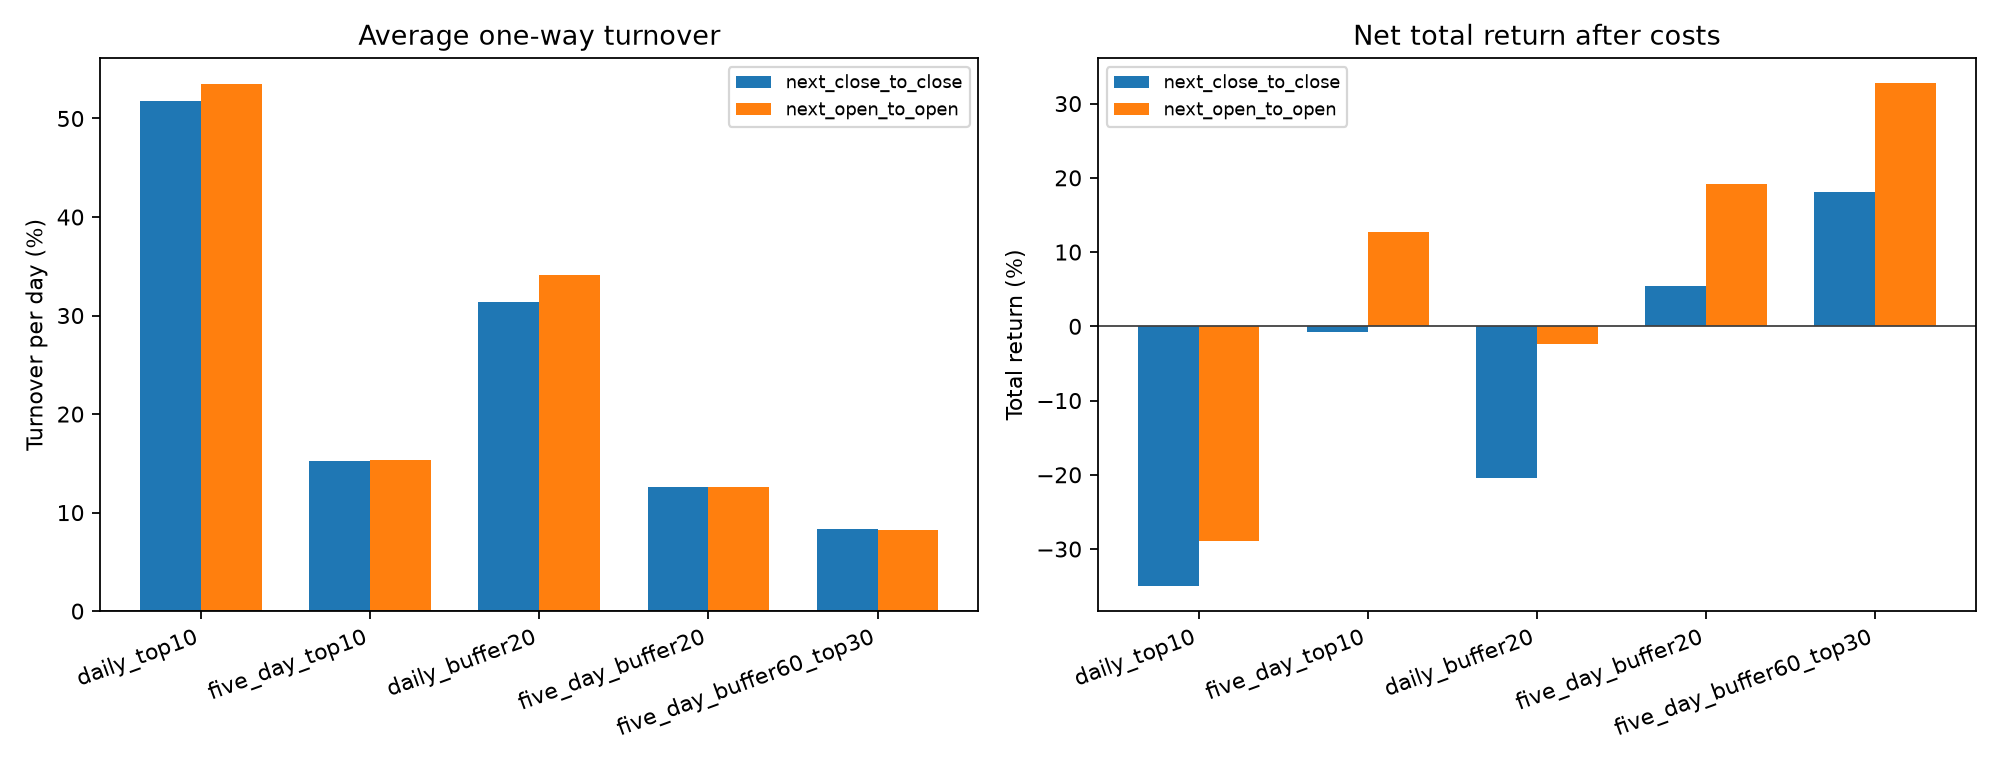
\includegraphics[width=0.96\textwidth]{qr_turnover_comparison.png}
\caption{不同换手控制政策比较。最终方案把次日开盘口径日均单边换手从 53.45\% 降至 8.27\%。}
\end{figure}

\section{步骤十：成交时点、限制与交易成本}

信号在 $t$ 日形成，只能在 $t+1$ 日开盘或收盘成交，随后持有到下一对应价格时点。成交量或成交额为零视为停牌；一字涨停不能买入，一字跌停不能卖出；无法卖出的股票继续保留。

成本由三部分组成：卖出金额的 5 个基点手续费；买卖双方各 5 个基点基础滑点；以及订单金额占当日成交额比例驱动的平方根冲击：
\begin{equation}
c^{impact}_{i,t}=\min\left(c_{max},\eta\sigma_{i,t}\sqrt{\frac{Q_{i,t}}{ADV_{i,t}}}\right).
\end{equation}
其中 $Q$ 为订单金额，$ADV$ 为日成交额，$\sigma$ 为波动尺度，$\eta$ 为冲击系数。该设计使低流动性股票和大额订单承担更高成本。

\chapter{风险收益结果与稳健性检验}

\section{步骤十一：绩效指标定义}

累计收益为 $\prod_t(1+r_t)-1$；年化收益为 $(1+R)^{252/T}-1$；年化波动率为 $\sigma(r)\sqrt{252}$；最大回撤为净值相对历史峰值的最小跌幅；夏普率为年化平均超额于无风险利率后的收益除以年化波动；信息比率为主动收益均值除以跟踪误差并年化。等权基准使用入场日可以买入股票的当日等权收益。

\begin{table}[H]
\centering
\caption{最终策略完整样本风险收益}
\begin{tabular}{lrr}
\toprule
指标 & 次日收盘 & 次日开盘 \\
\midrule
成本前累计收益 & 26.99\% & 42.63\% \\
成本后累计收益 & 18.15\% & \textbf{32.74\%} \\
年化收益 & 16.45\% & \textbf{29.51\%} \\
年化超额收益 & 12.63\% & \textbf{25.70\%} \\
年化波动率 & 18.52\% & 18.45\% \\
最大回撤 & -16.98\% & \textbf{-11.27\%} \\
夏普率 & 0.915 & \textbf{1.494} \\
信息比率 & 1.078 & \textbf{1.936} \\
日均单边换手 & 8.37\% & \textbf{8.27\%} \\
总交易成本 & 871,169 & 893,843 \\
\bottomrule
\end{tabular}
\end{table}

\begin{figure}[H]\centering
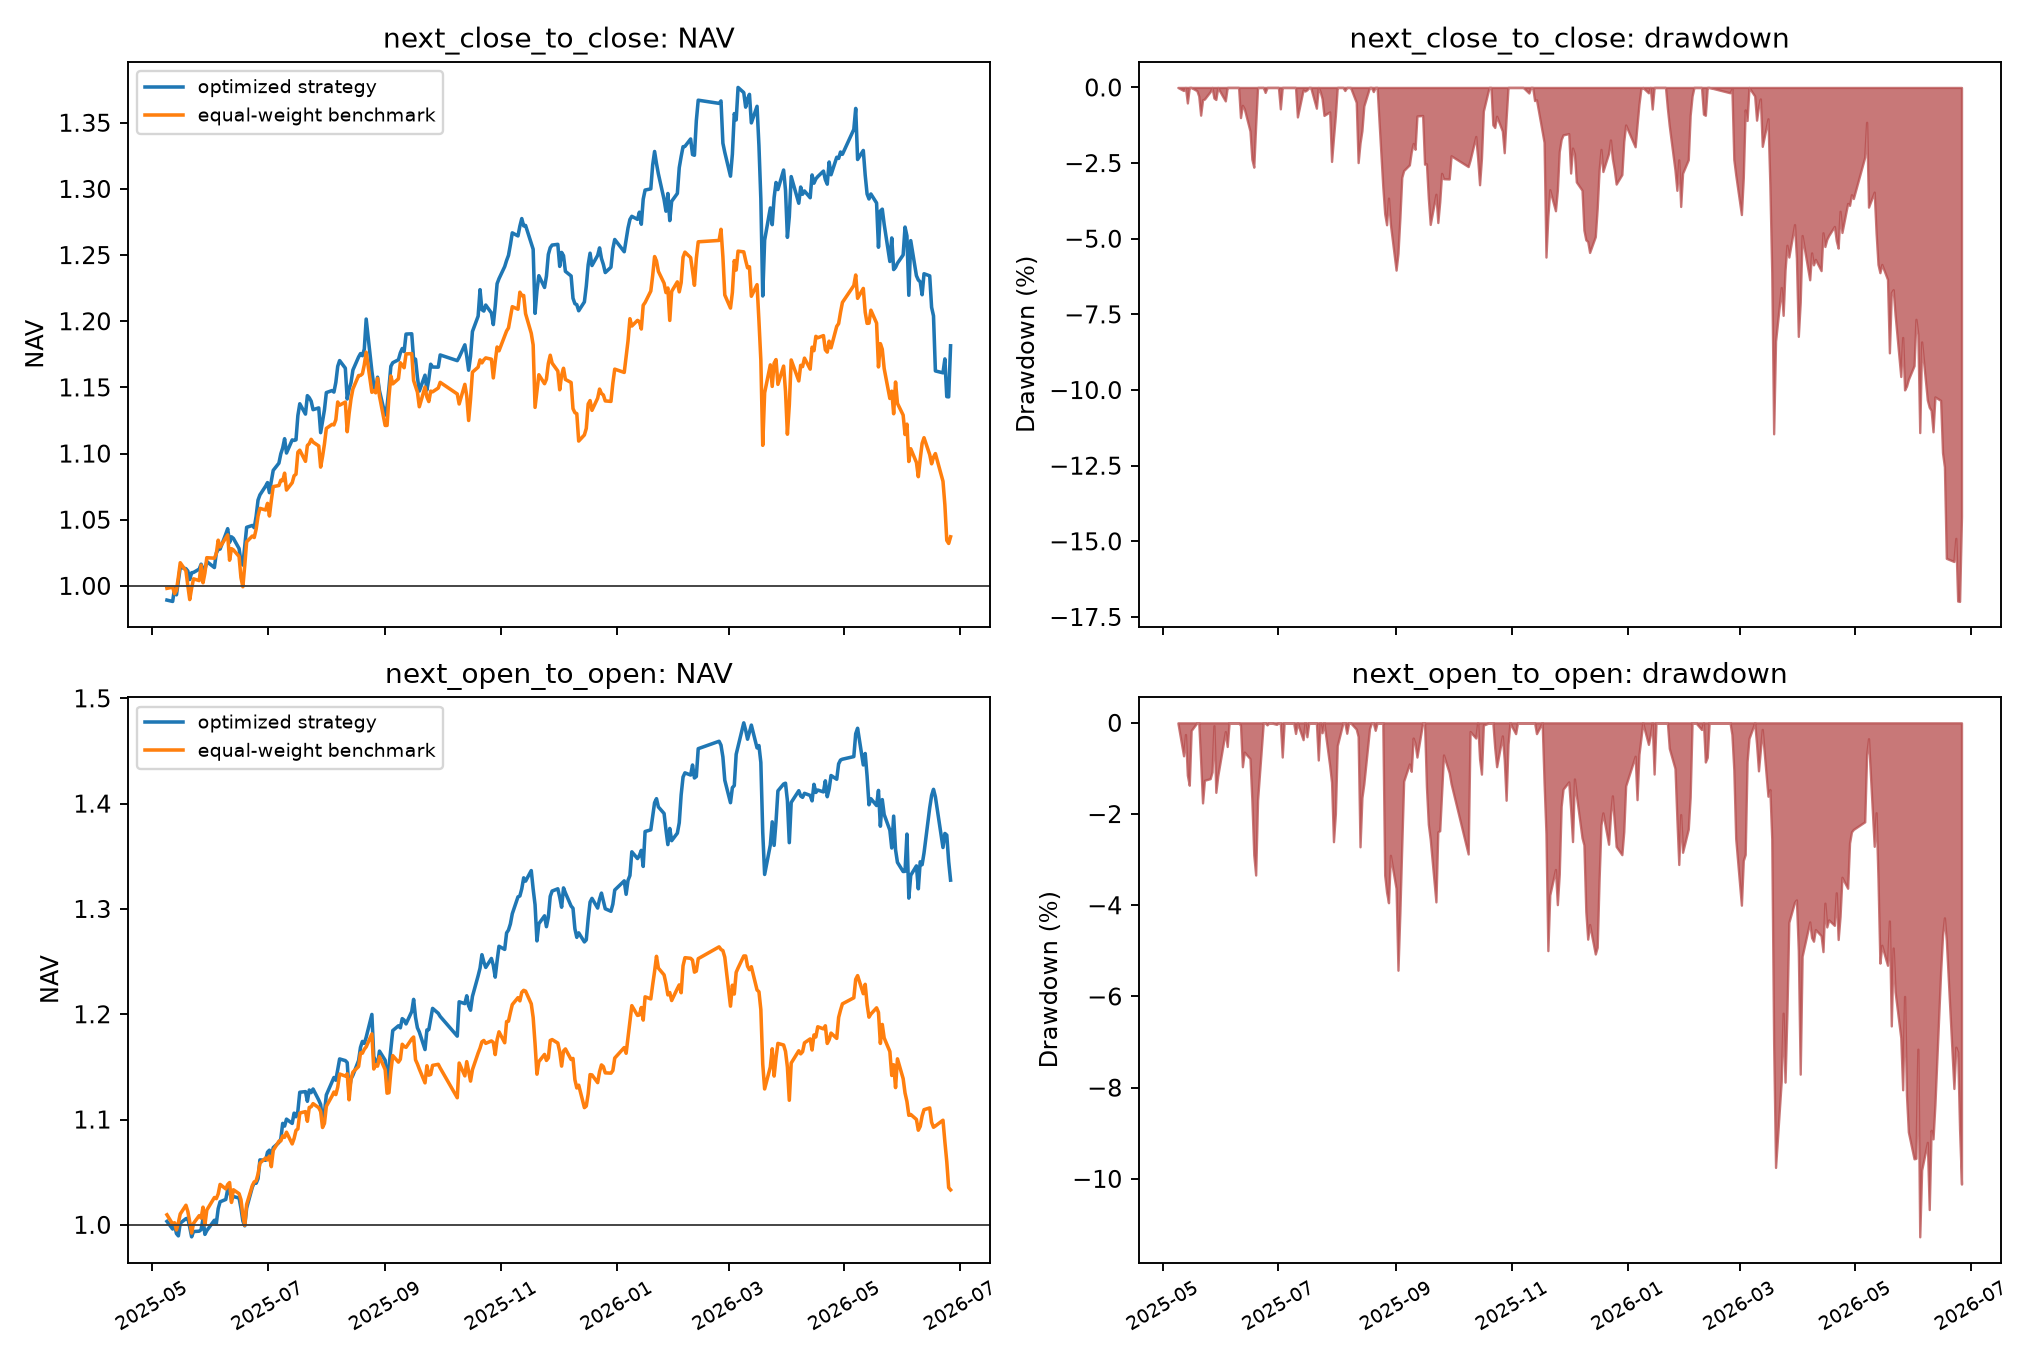
\includegraphics[width=0.98\textwidth]{qr_nav_drawdown.png}
\caption{正式七因子策略净值、等权基准与回撤。次日开盘结果在收益和回撤两方面优于次日收盘。}
\end{figure}

\begin{figure}[H]\centering
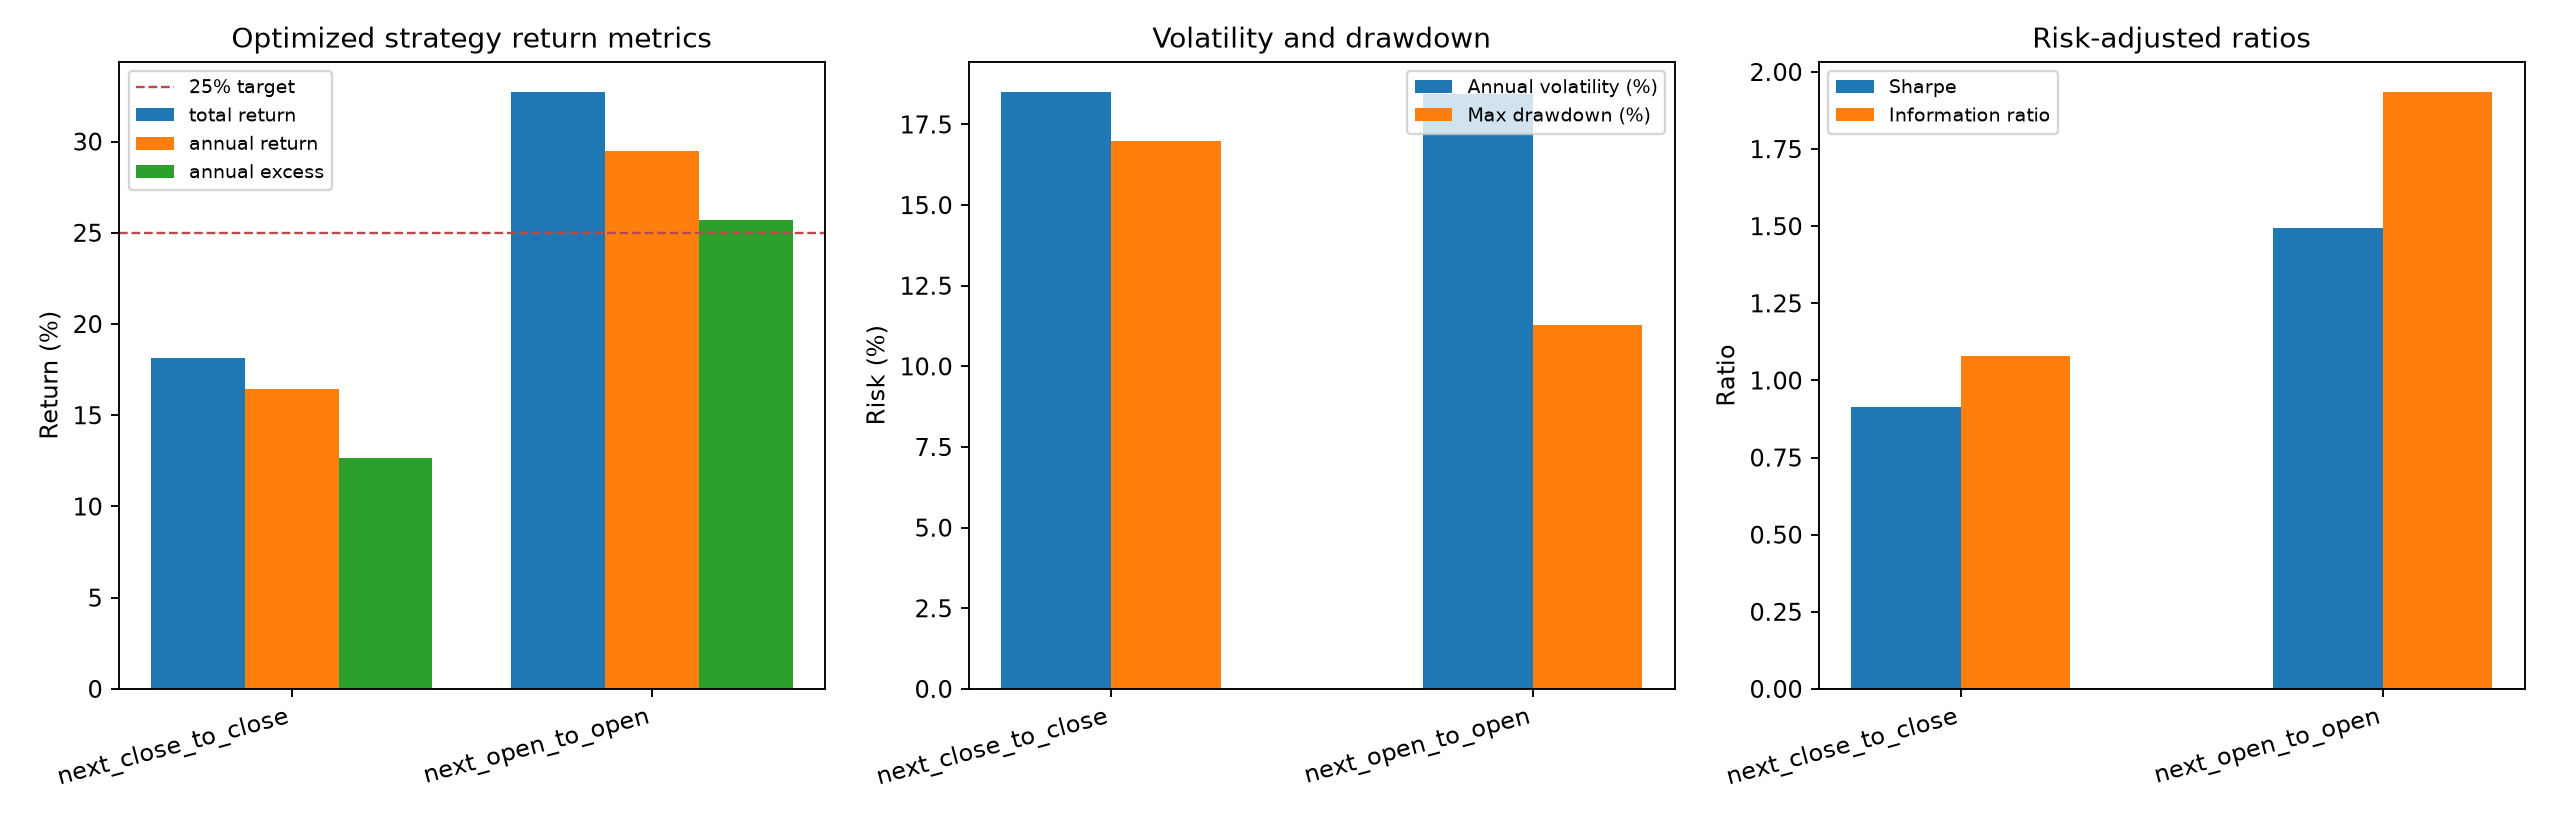
\includegraphics[width=0.96\textwidth]{qr_risk_metrics.png}
\caption{收益、波动、回撤、夏普率、信息比率和换手率的并列比较。}
\end{figure}

\section{步骤十二：成本敏感性}

乐观情景只保留卖出手续费；基准情景使用双边 5bp 滑点和当前平方根冲击模型；悲观情景使用双边 10bp 滑点并把冲击参数提高 50\%。次日开盘口径的净收益分别为 41.05\%、32.74\% 和 27.37\%。悲观情景仍超过 25\%，但结果明显随成本假设下降，说明流动性和执行质量仍是关键风险。

\begin{figure}[H]\centering
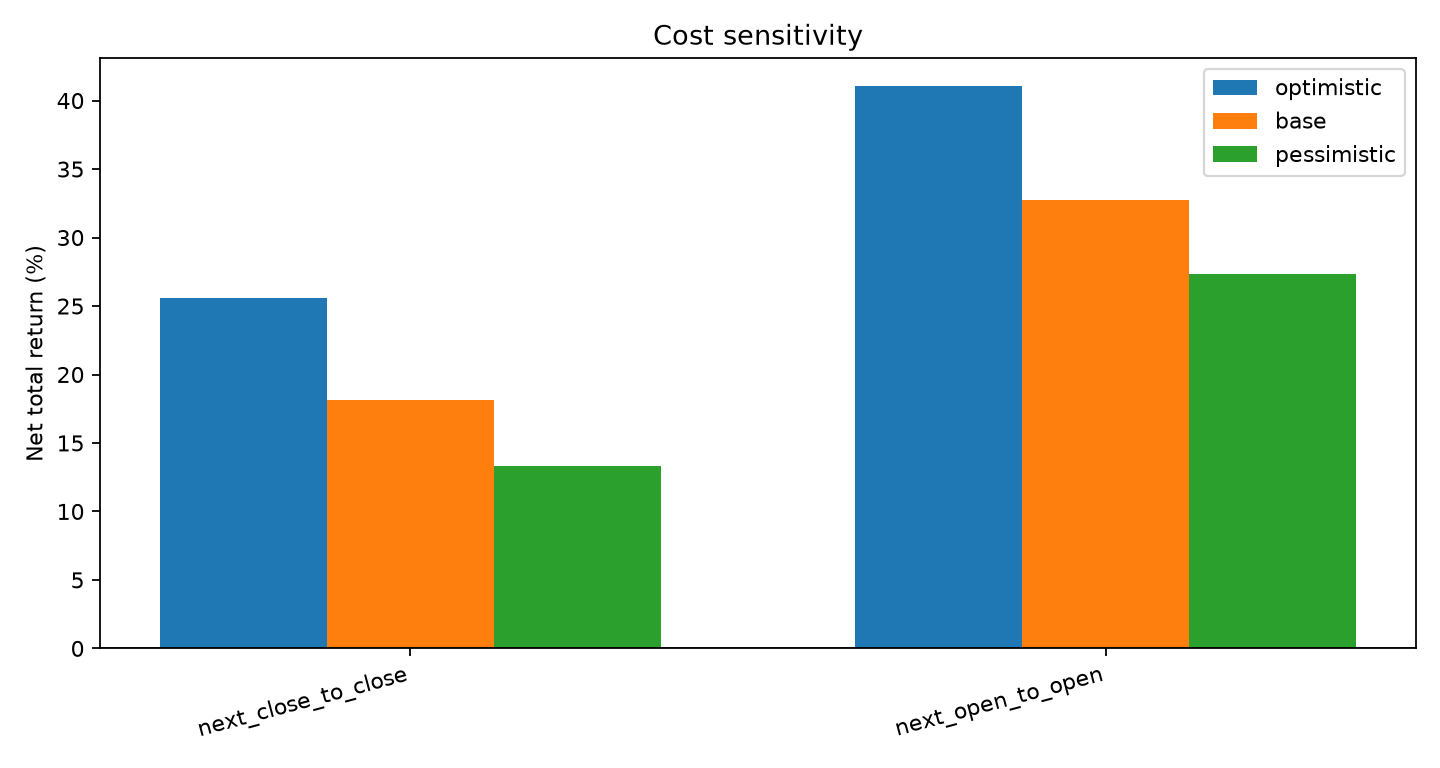
\includegraphics[width=0.90\textwidth]{qr_cost_sensitivity.png}
\caption{乐观、基准和悲观成本情景下的累计收益、夏普率与总成本。}
\end{figure}

\section{步骤十三：因子消融}

消融实验从一个因子逐步增加到七个因子，用于判断新增信号是否带来边际价值。次日开盘口径下，四个原有因子组合净收益为 31.14\%，七因子组合为 32.74\%；新增因子的价值主要体现在组合分散、回撤与风险调整后收益，而不是每增加一个因子都单调提高收益。

\begin{figure}[H]\centering
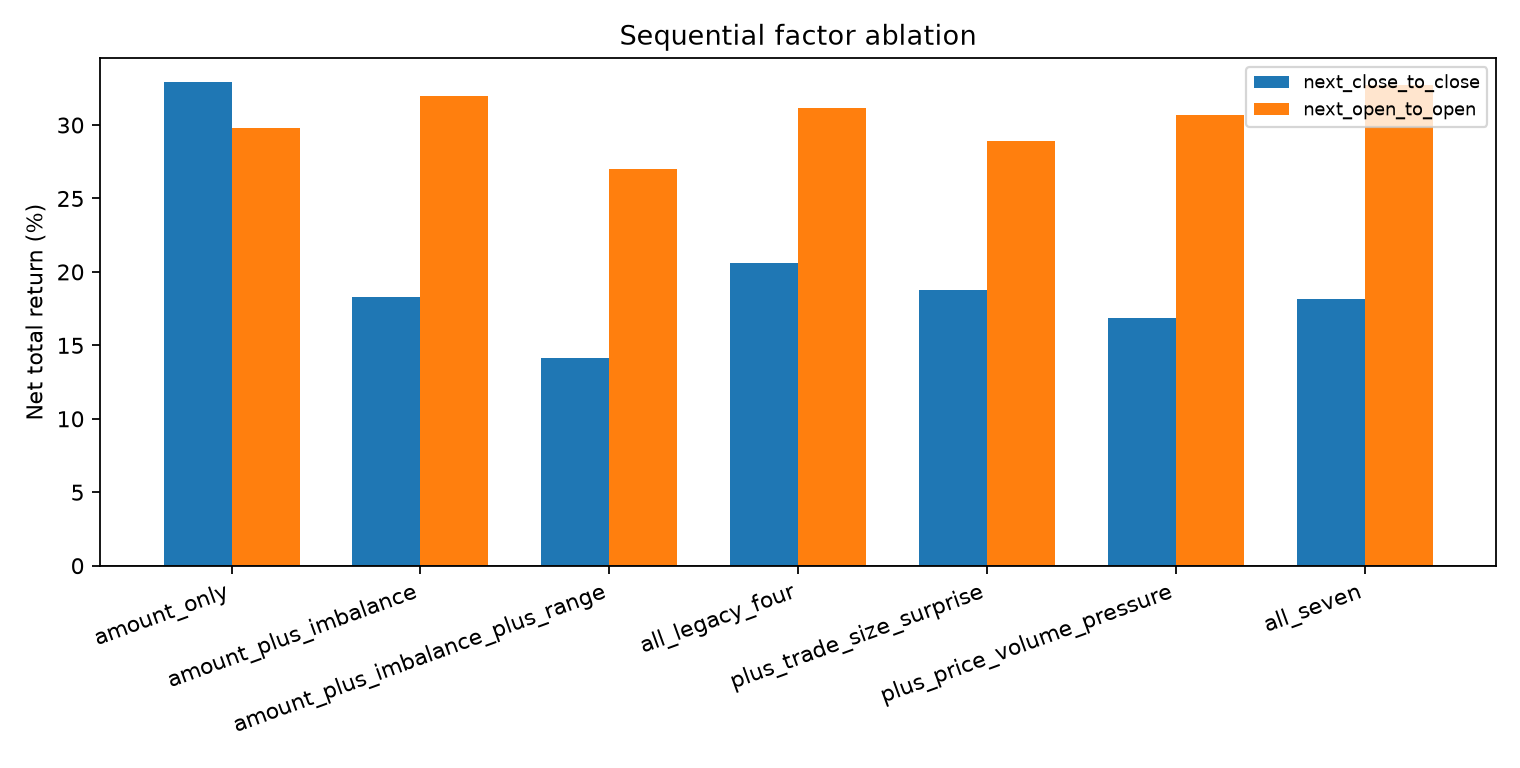
\includegraphics[width=0.94\textwidth]{qr_factor_ablation.png}
\caption{因子组合消融结果。多因子组合应同时比较 Rank IC、毛多空收益和执行成本后的策略收益。}
\end{figure}

\section{步骤十四：研究期与留出期}

为区分研究选择效应与时间外推能力，样本按时间切分为前 80\% 研究期和后 20\% 留出期。次日开盘策略在研究期累计收益 36.30\%，在留出期为 -2.61\%；同期留出期等权基准为 -7.61\%，因此累计主动收益仍为 5.41\%。这说明策略在下跌环境中相对抗跌，但尚未证明稳定的正绝对收益。

\begin{figure}[H]\centering
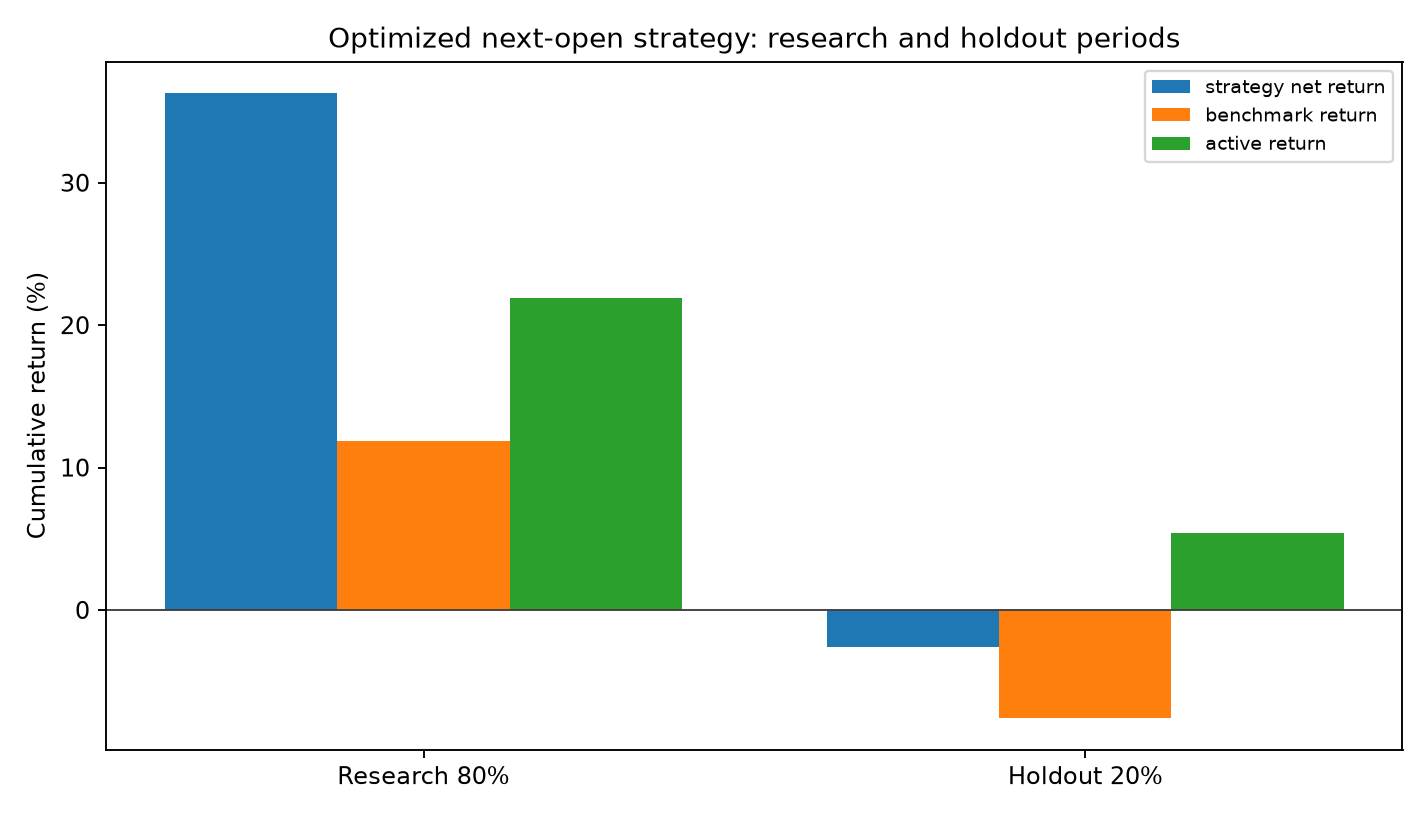
\includegraphics[width=0.96\textwidth]{qr_period_split.png}
\caption{完整样本、前 80\% 研究期与后 20\% 留出期比较。完整样本 32.74\% 不能替代独立样本外验证。}
\end{figure}

\chapter{多股票 Walk-forward LSTM}

\section{步骤十五：样本、特征与标签}

分钟模型选取 6 只股票和 140 个交易日，以过去 20 分钟预测下一分钟是否上涨。输入特征包括对数收益、分钟振幅、对数成交量、主动买卖不平衡和日内时间位置。标签定义为
\begin{equation}
y_{t+1}=\mathbb{I}(C_{t+1}>C_t).
\end{equation}
每个样本只包含预测时点及以前的信息，避免把下一分钟数据放入输入窗口。

\section{步骤十六：Expanding-window 验证}

模型采用单层 PyTorch LSTM，隐藏维度为 16。验证使用三折 expanding-window walk-forward：每折至少包含 60 个训练日、20 个验证日和 20 个测试日；标准化参数只用训练期估计，验证期负责选模，三个测试窗口互不重叠。合并后共有 83,880 条样本外预测，上涨样本占 31.09\%。

\begin{table}[H]
\centering
\small
\caption{样本外分类结果}
\begin{tabular}{lrrrrrrr}
\toprule
模型 & Acc. & Bal.Acc. & Prec. & Recall & F1 & ROC AUC & PR AUC \\
\midrule
多数类 & 68.91\% & 50.00\% & 0.00\% & 0.00\% & 0.00\% & 0.5000 & 0.3109 \\
逻辑回归 & 68.93\% & 51.23\% & 50.51\% & 4.40\% & 8.10\% & 0.6086 & 0.3993 \\
LSTM & 68.98\% & 52.28\% & 50.77\% & 8.10\% & 13.97\% & 0.6465 & 0.4276 \\
\bottomrule
\end{tabular}
\end{table}

\section{步骤十七：准确率诊断与解释}

图~\ref{fig:lstm-accuracy} 将合并样本外准确率与三折测试准确率放在同一张图中。LSTM 的总体准确率为 68.98\%，但上涨样本仅占 31.09\%，因此一个始终预测“下跌”的多数类模型也能得到 68.91\% 的准确率。LSTM 相对多数类基线只提高了 0.07 个百分点，不能把 68.98\% 直接解释为较强的方向预测能力。

相比之下，平衡准确率会分别计算上涨和下跌两类的召回率，再取平均。LSTM 的平衡准确率为 52.28\%，高于多数类的 50.00\% 和逻辑回归的 51.23\%，说明模型对少数类上涨样本提供了有限但为正的增量识别能力。三折测试准确率分别为 69.22\%、68.88\% 和 68.84\%，时间窗口之间较稳定，但仍与多数类基线非常接近。

\begin{figure}[H]\centering
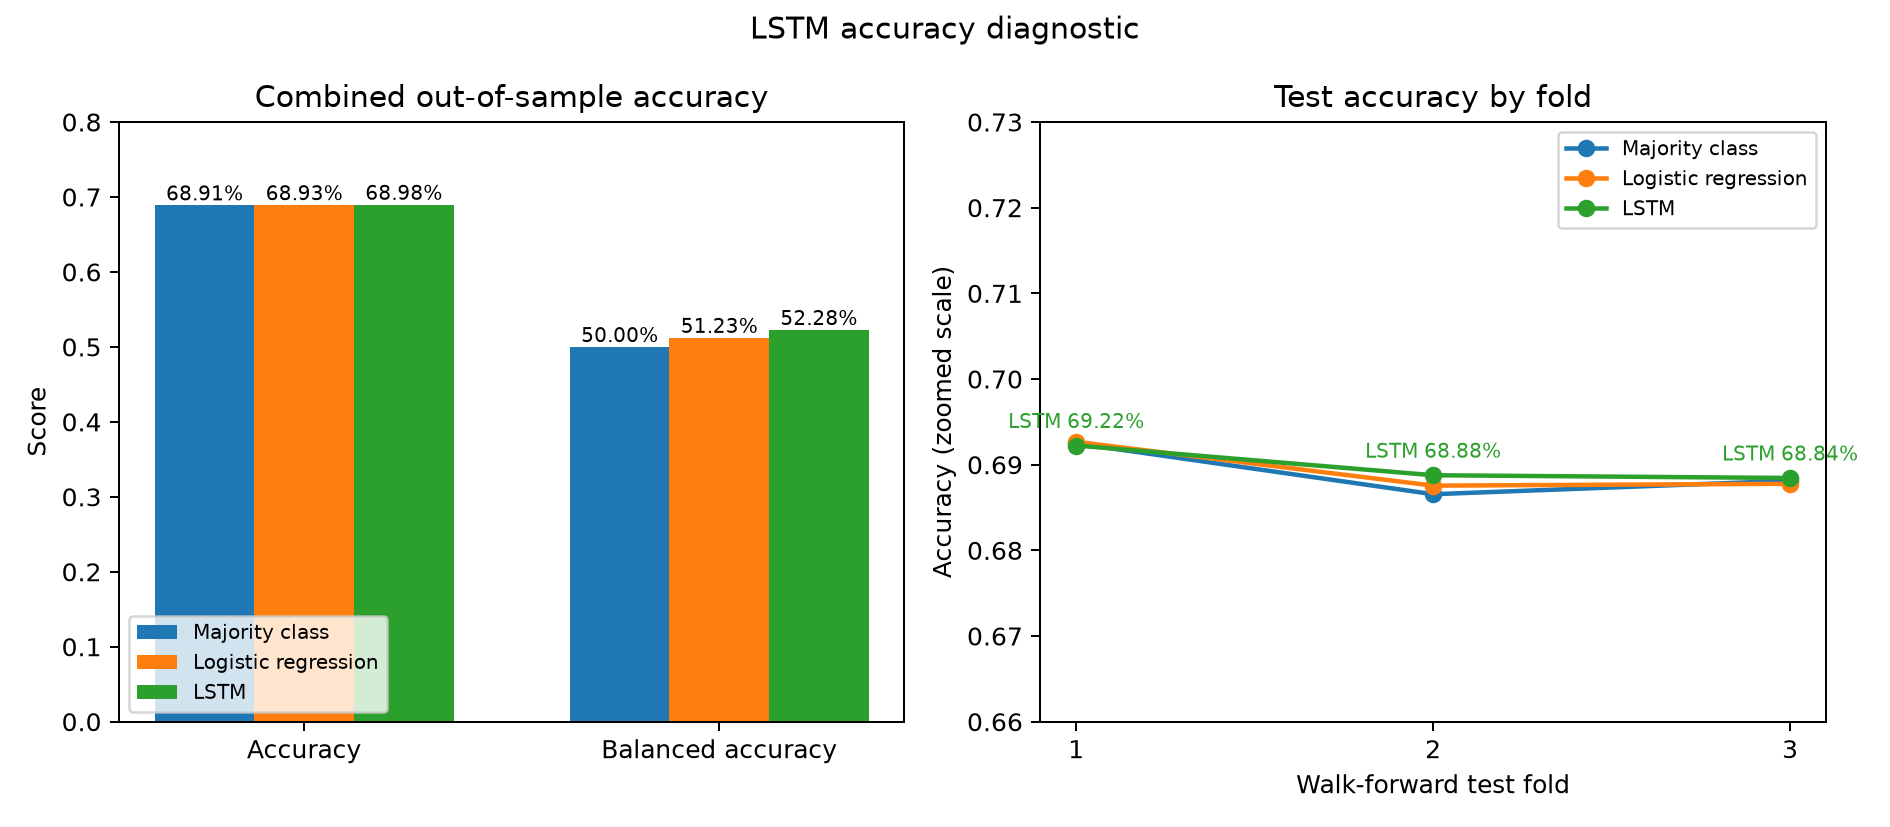
\includegraphics[width=0.98\textwidth]{qr_lstm_accuracy.png}
\caption{LSTM 准确率诊断。左图比较合并样本外 Accuracy 与 Balanced Accuracy；右图比较三折测试 Accuracy。由于类别不平衡，总体 Accuracy 必须与多数类基线、平衡准确率和排序指标一起解释。}
\label{fig:lstm-accuracy}
\end{figure}

结合上涨召回率 8.10\%、ROC AUC 0.6465 和 PR AUC 0.4276，可以得到更完整的结论：LSTM 的概率排序优于逻辑回归，但在 0.5 阈值下仍漏掉了大量上涨分钟。模型目前适合被描述为具有一定样本外排序信息，而不是已经形成高准确率或可直接交易的分钟策略。

\begin{figure}[H]\centering
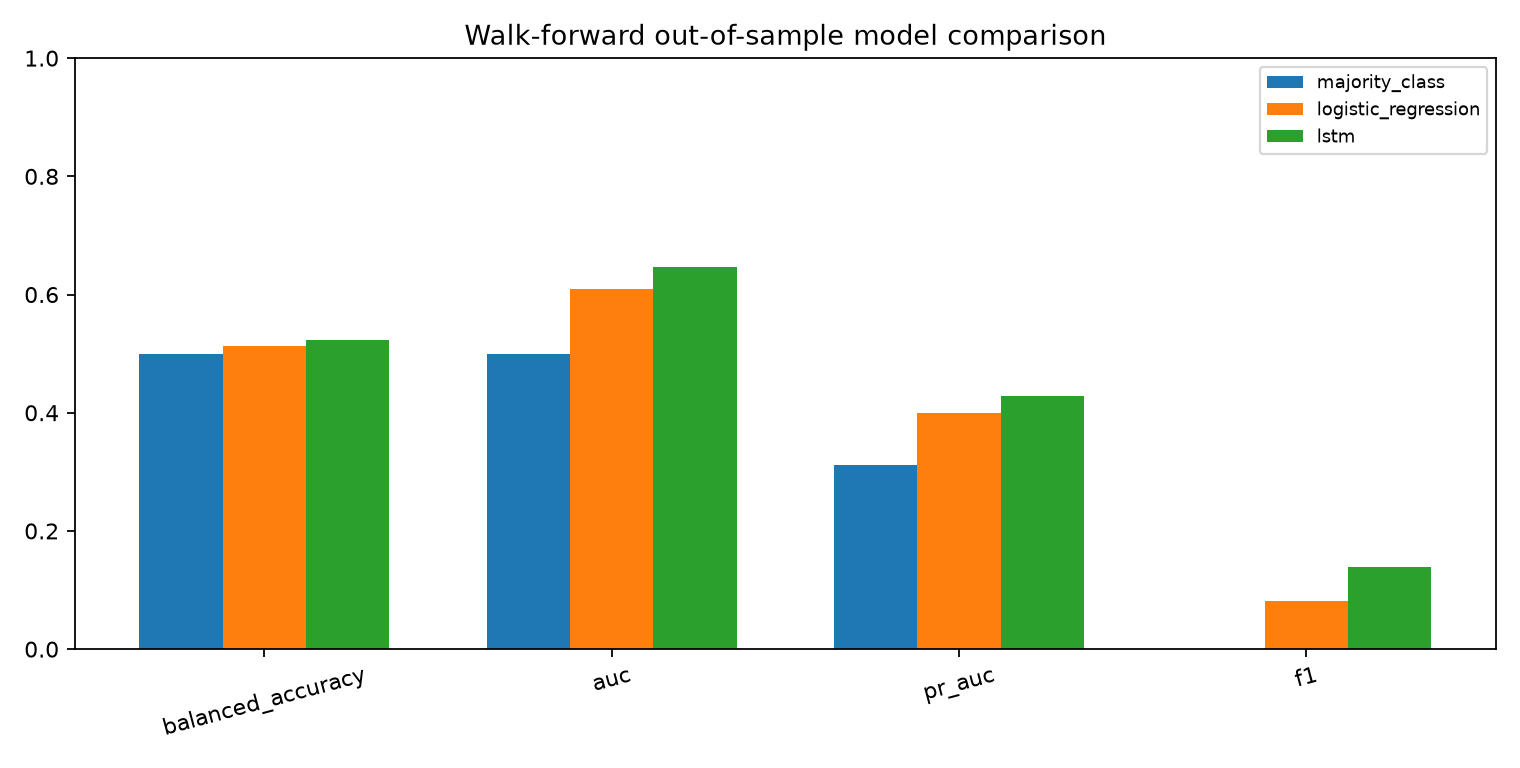
\includegraphics[width=0.88\textwidth]{qr_lstm_models.png}
\caption{多数类、逻辑回归和 LSTM 的样本外指标比较。LSTM 的排序指标高于逻辑回归。}
\end{figure}

\begin{figure}[H]\centering
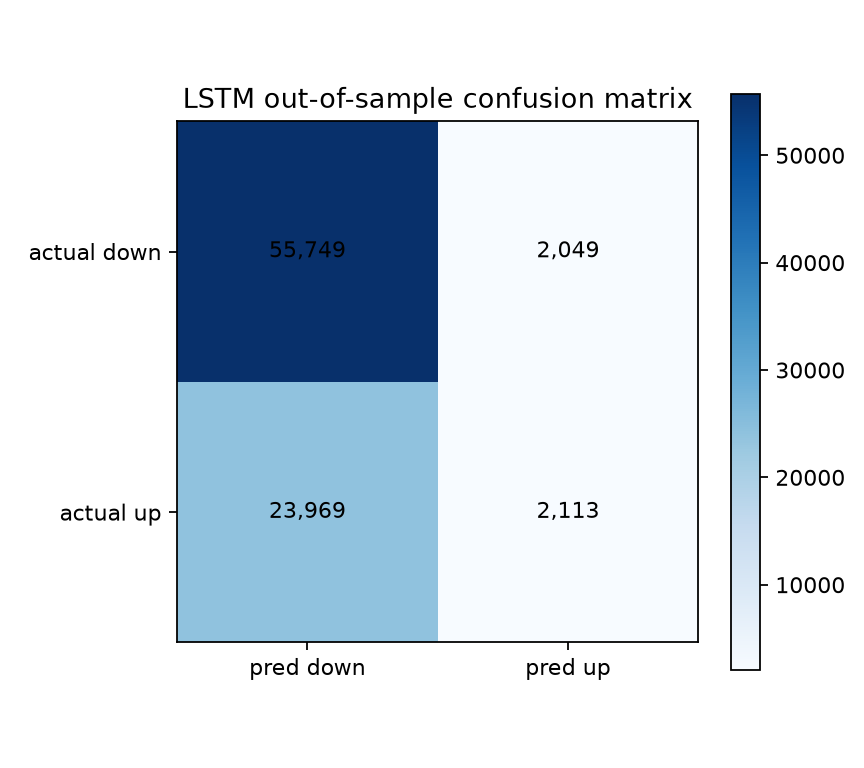
\includegraphics[width=0.72\textwidth]{qr_lstm_confusion.png}
\caption{LSTM 样本外混淆矩阵。真正例为 2,113，假负例为 23,969，说明 0.5 阈值下上涨召回率偏低。}
\end{figure}

\begin{figure}[H]\centering
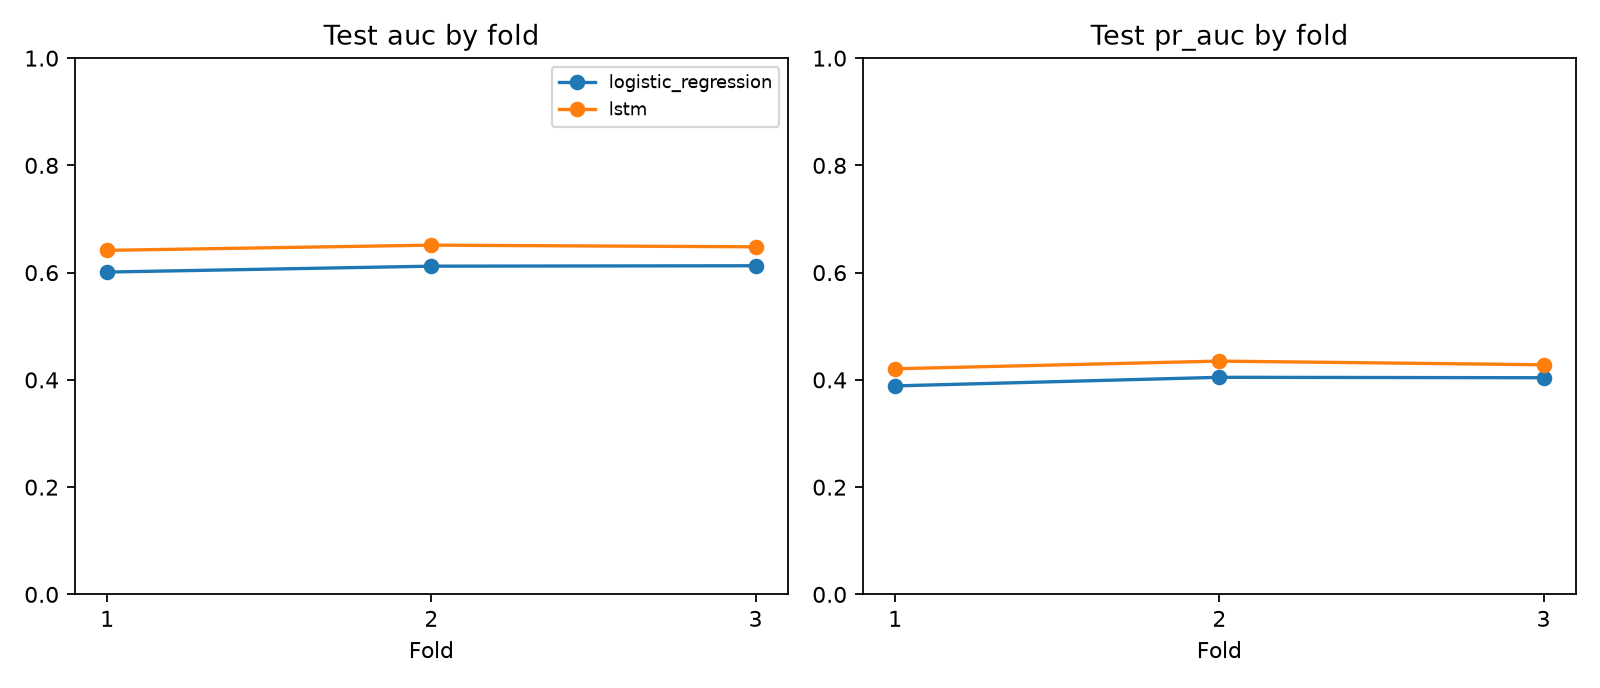
\includegraphics[width=0.92\textwidth]{qr_lstm_folds.png}
\caption{三折 walk-forward 的逐折指标。逐折结果可用于判断表现是否集中在某一时间窗口。}
\end{figure}

LSTM 的 ROC AUC、PR AUC 和 F1 均高于逻辑回归，说明序列结构提供了一定额外排序信息；但总体准确率几乎等于多数类基线，且上涨召回率仅 8.10\%。因此模型目前只能被解释为“具有样本外排序信息”，还不能直接被解释为“可交易的分钟策略”。下一步应进行概率校准、阈值选择、概率分组收益与分钟交易成本检验。

\chapter{结论、限制与下一步}

\section{主要结论}

\begin{itemize}
  \item 七个日频因子中，多数因子具有方向稳定的横截面信息；新增的单笔成交规模异常、价量压力和隔夜--日内背离没有复制参考材料中的因子。
  \item 历史 IC 加权避免了同日未来收益泄漏；Top30、每 5 日调仓和 Top60 缓冲把日均单边换手降至约 8.3\%。
  \item 次日开盘口径完整样本成本后累计收益为 32.74\%，年化收益为 29.51\%，年化超额收益为 25.70\%，最大回撤为 -11.27\%。
  \item 最后 20\% 留出期的绝对收益仍为负，表明完整样本结果含有研究选择效应，需要继续用全新的时间区间进行 walk-forward 检验。
  \item LSTM 的样本外排序指标高于逻辑回归，但 0.5 阈值下上涨召回率较低，尚未完成分钟交易层面的经济价值闭环。
\end{itemize}

\section{结果解释边界}

报告中的 25\% 以上收益来自指定历史样本和明确成本模型，不能被表述为收益保证。匿名股票代码导致真实行业、市值和可比市场指数不可获得，因此使用股票池内可交易股票的等权收益作为基准，并明确跳过行业与市值中性化。下一步最重要的工作是增加独立时间段、检查不同市场状态与流动性分组，并把 LSTM 概率转化为含成本的分钟交易实验。

\end{CJK*}
\end{document}
